% vim : tabstop 4
%%%%%%%%%
% manual_go.tex - Introducción a Go
% Roberto Costumero Moreno <roberto@costumero.es>
% Héctor Ambit Hernández <h.ambit.h@gmail.com>
%%%%%%%%%

% Tipo de documento
\documentclass[a4paper,titlepage,twoside,openright]{book}

% Márgenes de todas las hojas
\usepackage[left=1.7cm, right=2.2cm, top=1.5cm, bottom=2.4cm]{geometry}

% Importación de paquetes a usar
\usepackage[spanish]{babel}
\usepackage[utf8]{inputenc}
\usepackage{times}
\usepackage{fancyhdr}
\usepackage{graphicx}
\usepackage{float}
\usepackage{boxedminipage}
\usepackage{listings}
\usepackage[usenames,dvipsnames]{color}
\usepackage{hyperref}

% Cambiamos el tipo de los Capítulos
\usepackage{psboxit,pstcol}
\makeatletter
\def\thickhrulefill{\leavevmode \leaders \hrule height 1ex \hfill \kern \z@}
\def\@makechapterhead#1{%
  \reset@font
  \parindent \z@ 
  \vspace*{10\p@}%
  \hbox{%
    \vbox{%
	  \hspace{0pt}
	  {\LARGE \bfseries \@chapapp{}
            \strut \vrule height 1em depth 0pt width 0pt
            \thechapter}%
      \hrule height 0.4pt depth 0pt width \hsize
      \par
      \vskip 6pt%
      \hspace{20pt}%
      \parbox{20cm}{%
        \Huge \bfseries #1}%
      }%
    }%
  \vskip 50\p@
}

% Definimos las cabeceras y pies de página
\pagestyle{fancy}
\lhead{\leftmark}
\chead{}
\rhead{SECCIÓN \rightmark} %\bfseries Introducción a Go}
\lfoot{}
\cfoot{\thepage}
\rfoot{}
\renewcommand{\headrulewidth}{0.1pt}
\renewcommand{\footrulewidth}{0pt}

% Definimos nuevos colores
\definecolor{light-gray}{gray}{0.95}

% Ponemos el color de fondo a los trozos de código.
\lstset{backgroundcolor=\color{light-gray}, breaklines=true,
extendedchars=\true, inputencoding=utf8, showstringspaces=false, tabsize=4,
captionpos=b, numbers=left, texcl=true}
\renewcommand{\lstlistlistingname}{Índice de códigos}
\renewcommand{\lstlistingname}{Código}


%%%%%%%%%%%%%%%%%%%
% Nuevos comandos
%%%%%%%%%%%%%%%%%%%
% Nota
\newcommand{\nota}[1]{
	\begin{center}
	\begin{boxedminipage}{16cm}
		\begin{flushleft}
			%\includegraphics[width=0.7cm]{im/imagen_nota.eps}
			\textbf{Nota.-} \begin{small}#1\end{small}
		\end{flushleft}
	\end{boxedminipage}
	\end{center}
}

% Consejo
\newcommand{\consejo}[1]{
	\begin{flushleft}
	\begin{tabular}{lr}
	\includegraphics[width=0.7cm]{im/imagen_consejo}
	& \parbox{14cm}{\textbf{Consejo.-} #1}\\
	\end{tabular}
	\end{flushleft}
}

%% Ejemplo codigo
\newcommand{\codigo}[3]{
	\begin{flushleft}
		\begin{tabular}{|l|}
			\hline
			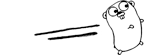
\includegraphics[width=1.5cm]{images/go_logo.png}
			\begin{large}\textbf{Ejemplo}\end{large}\\
		\end{tabular}
		\begin{tabular}{|cl|}
			\hline
			&\\
			&
			\begin{minipage}{16.2cm}
				\lstinputlisting[language=go,caption=#1,label=#2]{#3}
			\end{minipage} \\
			\hline
		\end{tabular}
	\end{flushleft}
}

%%%%%%%%%%%%%%%%%%%
% Comienzo del documento
\begin{document}

% Creamos el título
\title{
	{\Huge Introducción a Go}\\
	\ \\
	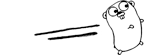
\includegraphics{images/go_logo.png}
	\author{\textbf{Roberto Costumero Moreno}\\
	\textbf{Héctor Ambit Hernández}
	}
}
\date{Noviembre 2011}
\maketitle
\newpage

% Creamos la página de la licencia
\thispagestyle{empty}
\textbf{\Large{Introducción a Go}}\\

Autores:\\

Roberto Costumero Moreno $<$roberto@costumero.es$>$

Héctor Ambit Hernández $<$h.ambit.h@gmail.com$>$\\

El logotipo de Go y la información correspondiente al presente manual ha sido obtenida, recopilada y modificada adecuadamente de la página oficial de Go, \textit{http://golang.org}.

El logotipo de Go y la información referente al lenguaje están licenciadas por Google\texttrademark\  bajo una \textbf{Licencia Reconocimiento 3.0 de Creative Commons} y puede consultarse en la siguiente dirección: \textit{http://creativecommons.org/licenses/by/3.0/es/}. El uso del logotipo y de la información están autorizados por la presente licencia mencionando su correcta atribución.

\begin{flushleft}

\includegraphics{images/cc.png}
\end{flushleft}

Esta obra puede ser distribuida únicamente bajo los términos y condiciones expuestos en la \textbf{Licencia Reconocimiento-No Comercial-Compartir bajo la misma licencia 3.0 España de Creative Commons} o superior (puede consultarla en \textit{http://creativecommons.org/licenses/by-nc-sa/3.0/es/}).\\

\clearpage
\thispagestyle{empty}
\begin{flushright}
Gracias a todos nuestros amigos y compañeros

que han hecho posible la publicación de este libro,

con su apoyo y comprensión en esos momentos de locura

y euforia con este gran lenguaje de programación.
\end{flushright}
\clearpage

\thispagestyle{empty}
\newpage

\pagenumbering{roman}

% Se crea el índice
\tableofcontents
\listoffigures
\listoftables
\lstlistoflistings
\newpage

\pagenumbering{arabic}

% Importamos cada uno de los capítulos creados en ficheros a parte.
% Capítulo 1: Introducción
\chapter{Introducción}

Este libro es el resultado del esfuerzo dedicado durante muchas horas a la
documentación del lenguaje de programación Go. Esta versión sustituye a todos
los efectos a la versión anterior desarrollada dentro del marco de un curso
ofrecido por uno de los autores para ACM Capítulo de Estudiantes en la Facultad de
Informática de la Universidad Politécnica de Madrid en el año 2010.\\

A través de los distintos capítulos, epígrafes y anexos se pretende iniciar al
lector en el lenguaje de programación Go, desarrollado por Google
\texttrademark, realizando una suave curva de iniciación e incluyendo una gran
cantidad de ejemplos explicativos, así como referencias a la documentación
oficial y herramientas que han sido también traducidas por los autores de este
libro.

El libro está dirigido a aquellas personas y programadores que tengan inquietud
por aprender este nuevo lenguaje de programación y que tienen una cierta base en
el mundo de la programación.

\section{¿Qué es Go?}

Go es un lenguaje de programación que fue presentado el 11 de Noviembre de 2009
y que originalmente estaba orientado a la programación de sistemas pero que ha
terminado siendo un lenguaje de programación de propósito general.\\

Según la página oficial \cite{Golang} es un lenguaje
expresivo, concurrente y que tiene recolector de basura. Además, presume de ser un
lenguaje simple, rápido, seguro, divertido y \emph{open
source}\footnote{Que el lenguaje sea \emph{Open Source} implica que cualquier
persona puede realizar modificaciones en el lenguaje o implementar nuevas
librerías que sean distribuidas como parte del mismo.}.\\

Go sigue una sintaxis bastante habitual en los lenguajes de programación más
usados, por lo que si se ha programado antes en C o Java la curva de aprendizaje
será mucho más suave.\\

Las principales características de Go son:

\begin{itemize}
	\item Es un lenguaje compilado muy, muy rápido.
	\item Usa una codificación UTF-8 para todos los ficheros fuente, es decir, permite usar
caracteres latinos, chinos, etc.  
	\item Usa tipado fuerte y memoria virtual segura.
	\item Posee punteros, pero no aritmética de los mismos.
	\item Es un lenguaje 100\% concurrente.
	\item Es Open Source, con lo que cualquier persona puede colaborar en su desarrollo
aportando ideas o implementando nuevas librerías.
	\item Por este último punto, posee una gran cantidad de librerías como, por
	ejemplo, un servidor web empotrado en el propio lenguaje.
\end{itemize}

\section{¿Quién lo desarrolla?}

Go es un proyecto promovido por cinco personas: Rob Pike, Robert Griesemer y Ken
Thompson, en primera instancia, a los que se unieron posteriormente Russ Cox
e Ian Lance Taylor. Todos los anteriormente citados, forman parte de
Google\texttrademark. Varios de ellos desarrollaron el Sistema Operativo
\emph{Plan 9} y han retomado muchas de las ideas originales para la creación
de este nuevo lenguaje de programación.

\section{¿Por qué crear un nuevo lenguaje?}

El lector podrá preguntarse cuál es la razón de crear un nuevo lenguaje de
programación, existiendo ya una gran variedad de lenguajes que permiten
desarrollar las técnicas de los grandes paradigmas de programación\cite{PVanRoy}.\\

Para empezar, el mundo informático ha avanzado enormemente en la última década,
a la par que no han aparecido nuevos lenguajes de programación que resuelvan las
nuevas casuísticas, como la programación web paralela o los problemas de
computación de altas prestaciones.\\

Actualmente, nos podemos encontrar las siguientes problemáticas que Go trata de
resolver de una manera eficiente:

\begin{itemize} 
	\item Los ordenadores son mucho más rápidos, pero no así el desarrollo de software. 
	\item Los sistemas software tienen una gran dependencia, por lo que a la
	hora de compilar es importante realizar un análisis eficiente de las
	dependencias entre los distintos ficheros, algo que no ocurre en los
	actuales ``ficheros de cabecera'' de C.
	\item Existe una tendencia creciente al uso de lenguajes de tipado dinámico,
	como Python y Javascript.
	\item La recolección de basura o la computación paralela, no están soportadas
	adecuadamente por los lenguajes de sistemas más populares.
	\item El aumento del número de núcleos en los ordenadores, ha provocado
	confusión y quebraderos de cabeza respecto a la programación concurrente y paralela. 
\end{itemize}

\section{Recursos}

Pese a que Go es un lenguaje moderno, ya existen numerosos sitios
de información sobre el lenguaje, aunque no siempre son fáciles de encontrar
debido a que el término ``Go'' es muy común en inglés. Por ello, la mayoría de
los desarrolladores de Go realizan búsquedas utilizando el término
\emph{golang}, que devuelve más y mejores resultados.

	\subsection{golang.org}
	
	El sitio web oficial del lenguaje, conviene recordar su dirección:
	\url{http://golang.org}. Toda la información que exista sobre el
	lenguaje se puede encontrar ahí, incluyendo enlaces a documentación externa
	aportada por miembros de la comunidad.\\
	
	Como curiosidad, cabe comentar que la propia página web está hecha en Go,
	utilizando el servidor web empotrado y una serie de templates HTML que trae
	``de serie''. A continuación, un repaso rápido a los sitios más importantes
	dentro de la página oficial:
	
	\begin{description} 
		\item[http://golang.org/doc] Acceso al listado de los ficheros de documentación.
		\item[http://golang.org/cmd] Acceso a la documentación sobre los comandos que pueden usarse.
		\item[http://golang.org/pkg] Acceso a la documentación de todos los paquetes existentes en Go.
		\item[http://golang.org/src] Acceso al código fuente de distintos
		ficheros de apoyo.
	\end{description}
	
	\subsection{blog.golang.org}

	El blog oficial de los desarrolladores del lenguaje. En él se van
	introduciendo entradas en las que se explican distintos aspectos del
	lenguaje de forma detallada, así como noticias que estén relacionadas con
	Go.

	\subsection{A tour of Go}

	En la dirección \url{http://go-tour.appspot.com} se encuentra una magnífica
	herramienta que permite introducir al programador en el lenguaje siguiendo
	un tutorial paso por paso. Esa es la versión original en inglés, pero se
	puede encontrar una versión traducida por los autores de este libro en
	\url{http://go-tour-es.appspot.com}

	\subsection{Lista de correo Go Nuts}
	
	La lista oficial de correo de Go se puede encontrar en la siguiente
	dirección:\\ \url{http://groups.google.com/group/golang-nuts}.
	Podrás darte de alta, ya que es una lista abierta, y recibir y enviar
	correos con todas las dudas que te surjan.

	\subsection{@go\_nuts}

	Existe una cuenta oficial del lenguaje en Twitter:
	\url[http://www.twitter.com/go\_nuts]{@go\_nuts} que suele publicar
	contenido interesante sobre Go.

	\subsection{\#go-nuts}
	
	Existe un canal de chat oficial en IRC para discutir acerca del lenguaje. Si
	quieres realizar una sesión \emph{live} sobre Go, entra en el canal
	\textbf{\#go-nuts} en el servidor \url{irc.freenode.net}.
	
	\subsection{Gestor de errores}
	
	Hay una página dedicada a gestionar todos los posibles errores del lenguaje,
	para ser así resueltos de forma eficiente. Es una página web pública y se
	puede encontraren: \url{http://code.google.com/p/go/issues/list}.
	
	\subsection{http://go-lang.cat-v.org/}
	
	Un sitio web mantenido a partir de todas las aportaciones de la gente
	a través de la lista de correo oficial. Contiene muchas librerías
	actualmente en desarrollo, ports del lenguaje a otros entornos, y sobre
	todo, archivos de coloreado de código fuente para una gran cantidad de
	programas de edición de texto.	

\section{¿Cómo instalar Go?}

Para instalar todas las librerías de Go y las herramientas propias del lenguaje,
hay que seguir unos sencillos pasos. En las próximas dos secciones se podrá ver
cómo instalarlo en sistemas UNIX y en sistemas Windows.

\subsection{Instalación en sistemas UNIX}

	Originalmente Go fue lanzado de manera exclusiva para sistemas UNIX. Aquí se
	describen los pasos necesarios para su instalación tanto en entornos Linux
	como Mac OS X y otros derivados de UNIX.

	Comenzamos con la inicialización de las variables de entorno necesarias para
	que la instalación se realice de forma correcta. Esta inicialización debería
	realizarse en ficheros de configuración dependientes del tipo de terminal
	usado, siendo para bash típicamente el fichero \emph{.bashrc}.

	\begin{enumerate} 
		\item Inicializar la variable \$GOROOT que indica el directorio raíz de Go. 
		Típicamente es el directorio \$HOME/go, aunque puede usarse cualquier otro.
		\item Inicializar las variables \$GOOS y \$GOARCH. Indican la
		combinación de Sistema Operativo y Arquitectura utilizada. Los posibles
		valores son los que se observan en la tabla \ref{Tabla_entorno}.
	
		\begin{table}[] 
			\begin{center} 
				\begin{tabular}{ccc} 
					\textbf{\$GOOS}	& \textbf{\$GOARCH} & \textbf{SO y Arquitectura}\\
					\hline 
					darwin & 386 & Mac OS X 10.5 o 10.6 -  32-bit x86\\
					darwin & amd64 & Mac OS X 10.5 o 10.6 - 64-bit x86\\ 
					freebsd & 386 & FreeBSD - 32-bit x86\\
					freebsd & amd64	& FreeBSD - 64-bit x86\\
					linux & 386 & Linux - 32-bit x86\\ 
					linux & amd64 & Linux - 64-bit x86\\
					linux & arm & Linux - 32-bit arm\\
					nacl & 386 & Native Client - 32-bit x86\\
				\end{tabular} 
			\end{center}
			\caption{Tabla de valores de \$GOOS y \$GOARCH.\label{Tabla_entorno}} 
		\end{table}
	
		\item Inicializar la variable \$GOBIN (opcional), que indica dónde serán
		instalados los binarios ejecutables. Por defecto es \$GOROOT/bin. Tras la
		instalación, es conveniente agregarla al \$PATH, para poder usar las
		herramientas desde cualquier directorio. 
	\end{enumerate}

	\nota{Hay que tener en cuenta que las variables \$GOOS y \$GOARCH
	indican el sistema contra el que se va a programar, no el sistema sobre el que
	se está programando, que estará definido por la variable \$GOHOSTOS, que
	aunque típicamente sea el mismo, no tiene por qué serlo.
	Es decir, estaremos todo el rato realizando una compilación
	cruzada.\footnote{Una compilación cruzada es aquella que se realiza cuando
	los ficheros binarios generados van a ser ejecutados en una máquina que
	posee una Arquitectura o Sistema Operativo distinto a la máquina sobre la
	que se desarrolla.}}

	Todo lo anterior se resume editando el fichero .bashrc, o cualquiera
	equivalente, añadiendo al final del fichero las siguientes líneas, con la
	configuración correcta:

\begin{lstlisting}[numbers=none]
export GOROOT=$HOME/go
export GOARCH=amd64
export GOOS=linux
export GOBIN=$GOROOT/bin
\end{lstlisting}

	Para bajarse las herramientas del repositorio, hay que tener instalado mercurial
	(tener el comando \emph{hg}). Si no se tiene instalado mercurial, se puede
	instalar con el siguiente comando:

\begin{lstlisting}[numbers=none]
$ sudo easy_install mercurial
\end{lstlisting}

	Si no se consigue instalar, conviene visitar la página oficial de descarga de
	mercurial.\footnote{http://mercurial.selenic.com/wiki/Download}\\

	Tras asegurarnos de que la variable \$GOROOT apunta a un directorio que no
	existe o que se encuentre vacío, hacemos un \emph{checkout} del repositorio
	con el comando:

\begin{lstlisting}[numbers=none]
$ hg clone -r release https://go.googlecode.com/hg/ $GOROOT
\end{lstlisting}

	Una vez que nos hemos bajado todos los ficheros necesarios, hay que instalar Go.
	Para ello hay que compilar el código fuente que nos hemos descargado
	y necesitaremos una serie de herramientas. A saber:

	\begin{itemize}
		\item GCC
		\item La biblioteca estándar de C
		\item Bison
		\item GNU make (versión $>=$ 3.81)
		\item awk
		\item ed
	\end{itemize}

	En entornos Mac OS X estas herramientas se pueden conseguir instalando el
	paquete XCode\cite{XCode}.

	El entornos Linux la instalación de estos paquetes dependerá de la
	distribución utilizada. En distribuciones basadas en Debian, se puede
	ejecutar el siguiente comando:

\begin{lstlisting}[numbers=none]
$ sudo apt-get install awk bison gcc libc6-dev ed make
\end{lstlisting}

	Para realizar la compilación e instalación de Go en base a las variables de
	entorno que definimos anteriormente, basta con ejecutar:

\begin{lstlisting}[numbers=none]
$ cd $GOROOT/src
$ ./all.bash
\end{lstlisting}

	Si la ejecución de \emph{all.bash} funciona correctamente, finalizará
	imprimiendo como últimas líneas:

\begin{lstlisting}[numbers=none]
--- cd ../test
N known bugs; 0 unexpected bugs

ALL TEST PASSED

---
Installed Go for linux/amd64 in /home/go.
Installed commands in /home/go/bin.
The compiler is 6g.
\end{lstlisting}

	donde N es un número que varía de una distribución a otra de Go, indicando bugs
	conocidos pero que no han podido ser arreglados. En la sección
	\ref{manteniendose} hablaremos sobre las distintas distribuciones de
	Go.

	Además, si estamos en Mac OS X habrá que ejecutar el comando
	\emph{./sudo.bash} para instalar los depuradores.

	\subsection{Instalación en sistemas Windows}

	La mejor forma de conseguir tener un entorno de desarrollo de Go en Windows es
	utilizar el entorno MinGW\cite{MinGW}. MinGW, de forma similar a Cygwin, simula
	un entorno tipo UNIX en sistemas operativos Windows, pero no intenta emular un
	entorno POSIX, sino que en su lugar utiliza el \emph{runtime} de C y la API de
	Windows\cite{MiekGieben}.

	Se puede por tanto instalar siguiendo los siguientes pasos, extraídos de
	\cite{MiekGieben}:

	\begin{itemize}
		\item Descargamos la última versión de MinGW de \cite{MinGW}.
		\item Extraemos los ficheros en nuestro disco C:\textbackslash.
		\item Aseguramos que los ficheros están en C:\textbackslash MingGW.
		\item Creamos un fichero dentro del directorio C:\textbackslash MinGW
		llamado \emph{setup.sh}, con el siguiente contenido:

\begin{lstlisting}[numbers=none]
export GOROOT=/c/go
export GOBIN=$GOROOT/bin
export PATH=$PATH:$GOBIN
\end{lstlisting}

		\item Ejecuta el acceso directo \emph{mintty} para lanzar una ventana de
		terminal.
		\item Cada vez que ejecutemos \emph{mintty}, podemos inicializar
		fácilmente nuestro entorno de desarrolo de Go ejecutando:

\begin{lstlisting}[numbers=none]
$ . ./setup.sh
\end{lstlisting}

		\item Descargamos la última versión estable de Go con el siguiente
		comando:

\begin{lstlisting}[numbers=none]
$ hg clone -r release https://go.googlecode.com/hg/ $GOROOT
\end{lstlisting}

		\item Al igual que en la versión UNIX, compilamos el código fuente para
		tener todo listo.

\begin{lstlisting}[numbers=none]
$ cd $GOROOT/src
$ ./all.bash
\end{lstlisting}

	Si la ejecución de \emph{all.bash} funciona correctamente, finalizará
	imprimiendo como últimas líneas:

\begin{lstlisting}[numbers=none]
--- cd ../test
N known bugs; 0 unexpected bugs

ALL TEST PASSED

---
Installed Go for linux/amd64 in /home/go.
Installed commands in /home/go/bin.
The compiler is 6g.
\end{lstlisting}
	\end{itemize}

\section{Manteniéndose al día\label{manteniendose}}

Go es un lenguaje moderno que se actualiza periódicamente. Para mantenerse al
día y conseguir que tu distribución funcione correctamente, hay que actualizar
cada vez que salga una nueva distribución, que se anuncia en la lista de correo
oficial de Go. Para actualizar a la última distribución disponible, hay que
ejecutar los siguientes comandos:

\begin{lstlisting}[numbers=none]
$ cd $GOROOT/src
$ hg pull
$ hg update release
$ ./all.bash
\end{lstlisting}

En Go existen diferentes distribuciones dependiendo del tipo de usuario al que
van dirigidas. Este libro está basado en la última versión release (r.60.3), que
es la recomendada para el público general. Las distribuciones de Go se
clasifican de la siguiente forma:

\begin{description}
	\item[Release] Es la versión más estable de Go. Se actualiza aproximadamente
	cada dos meses y es la recomendada para el público general.
	\item[Weekly] Es la versión más utilizada por los desarrolladores de
	bibliotecas del lenguaje. Se actualiza semanalmente y es propensa a errores,
	por lo que no es la más aconsejable salvo que desarrolles módulos del propio
	lenguaje.
	\item[Tip] Es la versión para los arriesgados. La que se actualiza con cada
	cambio realizado en el lenguaje y la más propensa a errores. Su uso está
	totalmente desaconsejado salvo que se necesiten los últimos cambios en el
	nucleo del lenguaje.
\end{description}

Si se quiere cambiar de una distribución a otra, se puede realizar mediante el
comando \emph{hg update distro}, donde \emph{distro} será el nombre de la
distribución que se quiera utilizar.

\newpage

% Capítulo 2: Características y tipos básicos
\chapter{Características y tipos básicos}

En este capítulo el lector se introducirá de lleno en todos los aspectos básicos
del lenguaje, desde sus principales características a los tipos más básicos,
donde además podrá ver cómo compilar los ficheros fuente utilizando los
compiladores nativos de Go, así como mediante el uso de Makefiles.

\section{Nuestro primer programa: ¡Hola Mundo!}

Sin más preámbulos, y después de contar un poco qué es Go y por qué se ha
realizado este manual, vamos a ver nuestro primer programa en Go: el típico
¡Hola mundo!

\codigo{Hola Mundo}{holamundo}{caracteristicas/holamundo.go}

\section{Garbage Collector\label{Garbage Collector}}

Go posee un Garbage Collector - Recolector de Basura - que identifica cuándo se
deja de utilizar una variable o una instancia concreta, y libera la memoria
asociada de forma automática.\\

Actualmente, el compilador de Go posee un Garbage Collector muy simple pero
efectivo, basado en un ``marcado de barrido'', es decir, marca aquello que puede
ser eliminado, y cuando se activa, se borra.\\

Está en desarrollo un Garbage Collector mucho más avanzado basado en las ideas
del Garbage Collector de IBM\texttrademark
\cite{IBMGC}. Esta nueva
implementación pretende ser muy eficiente, concurrente y de baja latencia, con
lo que nada más detectar que algo sobra, se elimine.

\section{Las bases del lenguaje}

Go está basado en una sintaxis bastante típica en los lenguajes de programación
modernos, con lo que cualquier conocimiento previo de lenguajes como C, serán de
mucha utilidad para seguir el libro.\\

Los ficheros fuente están codificados en UTF-8, lo que implica la posibilidad de
usar cualquier tipo de caracteres tanto latinos, como árabes o chinos en un
mismo fichero fuente, sin ningún tipo de limitación. Los delimitadores de las
declaraciones - o lo que es lo mismo, espacios en blanco no significativos - son
tres: espacios, tabulaciones y saltos de línea.\\

Los identificadores de cualquier variable en un programa escrito en Go, deben de
ser alfanuméricos, incluyendo el caracter `\_', teniendo en cuenta que las
letras y números deben ser aquellas definidas por
Unicode\footnote{\url{http://unicode.org}.}.

\section{Comentarios}

Los comentarios son exactamente los mismos que en C++. Para obtener un
comentario de una línea, utilizamos la combinación de caracteres \emph{//}, mientras
que para un comentario de varias líneas, se usa la combinación \emph{/* */}.

\begin{minipage}{17.1cm}
\begin{lstlisting}[language=go,numbers=none, caption=Comentarios correctos,
label=comentarioscorrectos]
// Esto es un comentario de una linea
/* Esto es un comentario que ocupa mucho
   y se parte en dos lineas. */
\end{lstlisting}
\end{minipage}

Hay que recordar, que los comentarios de varias líneas, no admiten anidamiento,
así pues, el siguiente comentario sería erróneo:

\begin{minipage}{17.1cm}
\begin{lstlisting}[language=go,numbers=none, caption=Comentario incorrecto,
label=comentarioincorrecto]
/* Esto es un comentario que ocupa varias lineas incorrecto.
   /* Con otro comentario anidado de varias lineas, que no es posible hacer.
   	*/
 */
\end{lstlisting}
\end{minipage}

\section{Literales}

Entendemos por \emph{literales} todas aquellas expresiones que representan un
valor concreto, ya sea en forma de cadena de caracteres o en forma numérica.\\

Existen tres tipos de valores literales en Go:

\begin{itemize}
	\item \textbf{Números:} Son aquellos números literales que representan un
	valor concreto sin necesidad de indicar su tamaño.
\begin{minipage}{17.1cm}
\begin{lstlisting}[language=go,numbers=none]
98
0x0FF
2.643e5
\end{lstlisting}
\end{minipage}

	\item \textbf{Strings:} Son aquellas cadenas de caracteres que pueden
	representarse en UTF-8 (o cualquier otra representación Unicode). También
	pueden representarse bytes con \emph{\textbackslash\textbackslash xNN} con
	2 dígitos o con \emph{\textbackslash\textbackslash 012} con 3 dígitos.

\begin{minipage}{17.1cm}
\begin{lstlisting}[language=go,numbers=none]
``Hola mundo\n''
``\\xFF''	// 1 byte
``\\u00FF''	// 1 caracter unicode, 2 bytes en UTF-8
\end{lstlisting}
\end{minipage}

	\item \textbf{Strings puros:} Son cadenas de caracteres que se imprimen tal
		cual son escritas en el código fuente, sin escapar ningún carácter. Se
		representan poniendo la cadena entre dos acentos graves ` \`\  '.

\begin{minipage}{17.1cm}
\begin{lstlisting}[language=go,numbers=none]
`\n\.abc\t\`  ==  ``\\n\\.abc\\t\\''
\end{lstlisting}
\end{minipage}
\end{itemize}

\section{Vistazo rápido de la sintaxis\label{sintaxis}}

La sintaxis de Go es una sintaxis muy familiar si se ha programado antes, aunque
tiene sus propias características y peculiaridades que conviene conocer, pero en
poco tiempo el lector debería reconocer este tipo de sintaxis.\\

A la hora de declarar una variable o un tipo se utiliza la palabra reservada
\emph{var}, seguida del identificador de la variable y terminando por el tipo de
la variable.\\

Veamos esto con un ejemplo, definiendo tres tipos de variables y un tipo \emph{Struct}.

\begin{minipage}{17.1cm}
\begin{lstlisting}[language=go,numbers=none]
var a int         // a es un entero
var b, c *int     // b y c son punteros a enteros
var d []int       // d es un array de enteros

// S es una estructura con dos atributos enteros.
type S struct {
    a, b int
}

var miVar S 	// miVar es una variable de tipo S
\end{lstlisting}
\end{minipage}

Las estructuras de control del programa, también nos resultarán familiares si
hemos trabajado con lenguages imperativos como C o Java, puesto que su
estructura es muy similar. Veamos un ejemplo con un \emph{if} y un \emph{for}.

\begin{minipage}{17.1cm}
\begin{lstlisting}[language=go,numbers=none]
if a == b {
    fmt.Print("a y b son iguales")
} else {
    fmt.Print("a y b son distintos")
}

for i = 0; i < 10; i++ {
	miVar++
}
\end{lstlisting}
\end{minipage}

\nota{En Go los paréntesis en las condiciones del \emph{if} o del
\emph{for} no hay que ponerlas. Sí que son siempre necesarias las llaves, que no
pueden ser omitidas. Además, hay que tener en cuenta que la llave de apertura de
un \emph{if} debe ir en la misma linea que la sentencia, y que el \emph{else},
si lo hubiera, tiene que ir emparejado en la misma linea que el cierre de bloque
del \emph{if}. En la sección \ref{if} en la página \pageref{if} se verá cómo es
la estructura correcta de estas sentencias de control.}

Por último hay que observar en el código anterior la ausencia del carácter `;' como
indicativo del final de sentencia.\\

Cuando Go fue creado, los puntos y coma eran obligatorios en todas las
instrucciones. Finalmente, se acordó que su uso sería opcional, y que sería el
propio compilador el que añadiría los puntos y coma al final de las sentencias
que considerara válidas. Aún así, el uso de puntos y coma en ciertas estructuras
es obligatorio, como puede ser en la separación de las distintas cláusulas de un
bucle \emph{for}.\\

Este esquema sigue las pautas acerca de este tipo de delimitadores del lenguaje
\emph{BCPL}, precursor de \emph{B} y por lo tanto de \emph{C}, y que Go ha decidido
adoptar.\\

Así pues, resumiendo acerca del uso de los puntos y coma:

\begin{itemize}
	\item Son opcionales en todos los programas al final de una sentencia,
	aunque deberían \textbf{no} ponerse. Únicamente son obligatorios a la
	hora de separar los elementos en la cláusula de un bucle \emph{for}
	o elementos en un \emph{if}.
	\item El compilador introducirá automáticamente los puntos y coma, por ello
	no es conveniente ponerlos, al final de una línea no vacía, si lo último que
	se encuentra es:
		\begin{itemize}
			\item Un identificador o un literal.
			\item Alguna de las palabras reservadas: break, continue,
			fallthrough o return.
			\item Alguno de los siguientes tokens: $++$, $--$, ), ], \}.
		\end{itemize}
		\item Se pueden poner los puntos y coma para separar instrucciones en
		una misma línea, pudiendo ser omitido antes de ')' o de '\}'.
\end{itemize}

\section{Tipos}

Go posee únicamente tres tipos básicos: Números, Booleanos y Cadenas de
caracteres.

	\subsection{Números}

	Existen tres tipos numéricos: Enteros, enteros sin signo y números
	flotantes.\\

	Cada uno de estos tipos tiene asociadas una serie de variantes dependiendo
	del número de bits en el que sea almacenado. El cuadro \ref{tiposnumericos}
	muestra un resumen con los tipos numéricos existentes.\\

	\begin{table}[htb]
		\begin{center}
			\begin{tabular}{ccc}
			\textbf{Enteros} & \textbf{Enteros sin signo} & \textbf{Flotantes}\\
			\hline
			int & uint & \\
			int8 & uint8 = byte & \\
			int16 & uint16 & \\
			int32 & uint32 & float32\\
			int64 & uint64 & float64
			\end{tabular}
		\end{center}
	\caption{Tabla de tipos numéricos}
	\label{tiposnumericos}
	\end{table}

	También existe el tipo \emph{uintptr}, que sirve para almacenar número
	enteros lo suficientemente grandes como para necesitar un puntero.\\

	Como puede deducirse de la tabla \ref{tiposnumericos}, el número que acompaña a cada
	nombre de tipo, es el número de bits que ocupa en memoria. Así, podemos
	observar que los números flotantes no tienen representaciones válidas con
	8 y 16 bits.\\

	Los tipos que no tienen asociado ningún número, \emph{int} y \emph{uint},
	se representan con un número de bits igual al ancho de la
	palabra de la máquina en la que se ha compilado el código. De esta forma se
	puede llegar a pensar que en un ordenador de 32-bit, los tipos \emph{int}
	e \emph{int32} son equivalentes, pero \textbf{no} es así. \textbf{Todos
	los tipos de la tabla son distintos}.\\

	Debido a que Go es un lenguaje con tipado fuerte\footnote{\textbf{Tipado
	fuerte}: Un lenguaje tiene tipado fuerte cuando todas las variables tienen
	que declararse con un tipo asociado, y no puede cambiar su tipo en tiempo de
	ejecución.}, no existe conversión implícita de tipos, aunque posteriormente
	veremos cómo pueden realizarse conversiones explícitas.

	\subsection{Bool}

	El tipo \emph{bool} define el tipo booleano usual, con dos constantes
	predefinidas que son: \emph{true} y \emph{false}.\\

	Hay que tener en cuenta, que a diferencia de otros lenguajes, en Go los
	\emph{punteros} y los \emph{enteros} \textbf{no son booleanos}.

	\subsection{String}

	El tipo \emph{string} representa un conjunto invariable de bytes, o lo que es
	lo mismo, texto tal y como lo entendemos. Los strings están delimitados por
	su longitud, no por un carácter nulo como suele ocurrir en la mayoría de
	lenguajes. Esto hace que el tipo \emph{string} sea mucho más seguro y eficiente.\\

	Toda cadena de caracteres representada por el lenguaje, incluidas las
	cadenas de caracteres literales, tienen como tipo \emph{string}.\\

	Como se ha dicho en el primer párrafo, y al igual que ocurre con los números
	enteros, los strings son invariables. Esto significa, que se pueden
	reasignar variables de tipo \emph{string} para que contengan otros
	valores, pero los valores de un literal de este tipo \textbf{no se pueden
	modificar}.\\

	De la misma forma que 5 siempre es 5, "Hola" siempre es "Hola".\\

	En otros lenguajes es posible modificar las cadenas de caracteres, ya sea
	dentro de una variable o de una constante, realizando un manejo explícito de
	la memoria. En Go y gracias a depender de su longitud, un string es
	invariable.\\

	Pese a que todo esto puede parecer incoherente o muy engorroso, las
	librerías de Go poseen un gran soporte para la manipulación de las cadenas
	de caracteres.

\section{Operadores}

	Los operadores en Go, como no podía ser de otra forma, son bastante comunes
	y la mayoría son utilizados en otros lenguajes. Existen operadores binarios,
	que reciben dos operandos, y operadores unarios.

	Tenemos varios tipos de operadores, que se pueden clasificar en 4 categorías
	distintas:

	\begin{itemize}
		\item Operadores aritméticos
		\item Operadores relacionales
		\item Operadores lógicos
		\item Operadores a nivel de bit
	\end{itemize}

	En los siguientes apartados vamos a ver cuáles son los operadores de los que
	disponemos y cuál es su precedencia a la hora de ser evaluados.

	\subsection{Operadores aritméticos}

	Los operadores aritméticos son aquellos que nos permiten realizar
	operaciones aritméticas sobre dos operandos. Son operadores que permiten
	realizar operaciones de suma, resta, multiplicación, etc.

	\begin{table}[htb]
		\begin{center}
			\begin{tabular}{ccccc}
				\textbf{Precedencia} & \textbf{Operador} & \textbf{Acción}
				& \textbf{Tipos de datos} & \textbf{Ejemplos}\\
				\hline
				2 & * & Multiplicación & enteros, reales, valores complejos & y = 2 * x\\
				2 & / & División & enteros, reales, valores complejos & y = x / 2\\
				2 & \ \% & Módulo & enteros & y = 3 \% 2\\
				2 & \& & AND a nivel de bit & enteros & y = 1 \& 1\\
				2 & \&\textasciicircum & Bit clear & enteros & y \& 3\\
				2 & $<<$ & Desplazamiento a la izquierda & entero $<<$ entero
				  sin signo & y = 2 $<<$ 1\\
				2 & $>>$ & Desplazamiento a la derecha & entero $>>$ entero sin
				  signo & y = 2 $>>$ 1\\
				1 & + & Suma & enteros, reales, valores complejos, strings & y = 3 + y\\
				1 & - & Resta & enteros, reales, valores complejos & y = 2 - x\\
				1 & \textbar & OR a nivel de bit & enteros & y = 1 \textbar\ 0\\
				1 & \textasciicircum & XOR a nivel de bit & enteros & y = 1 \textasciicircum 1\\
				\hline
			\end{tabular}
		\end{center}
		\caption{Tabla de operadores aritméticos}
		\label{tabopar}
	\end{table}

	La prioridad de los operadores determina cómo serán evaluados en una
	expresión sin paréntesis que delimite esa prioridad. Así pues, si hay dos
	operandos de distinta prioridad, se evaluará primero la operación de mayor
	prioridad. Si los operandos existentes son de la misma prioridad, la
	evaluación se realizará de izquierda a derecha.\\

	La columna \emph{Tipos de datos} de la tabla \ref{tabopar} indica sobre qué
	tipos de datos se pueden utilizar estos operadores.\\

	Los operadores \emph{+}, \emph{-} y \emph{\textasciicircum} pueden ser
	utilizados de forma unaria, recibiendo un único operando. Veamos esto con un
	pequeño ejemplo:

\begin{minipage}{17.1cm}
\begin{lstlisting}[language=go,numbers=none,caption=Ejemplo de operandos aritméticos unarios,label=oparitunarios]
+x 		// Implica 0 + x, o lo que es lo mismo, indicar que x es positivo.
-x 		// Implica 0 - x, o lo que es lo mismo, indicar que x es negativo.
^x 		// Es el complemento de x. Transforma los bits de x de 1 a 0 y los que estén en 0 a 1.
\end{lstlisting}
\end{minipage}

	\subsection{Operadores relacionales}

	Además de los operadores aritméticos, necesitamos una serie de operadores
	que nos permitan comparar dos valores para saber cuál es mayor que otro, si
	son iguales, etc. En este caso, los operadores relacionales nos aportan esta
	funcionalidad.\\

	En el caso de los operadores aritméticos existe una prioridad que determina
	qué operación se evalúa antes, pero eso no es necesario para los operadores
	relacionales que siempre se evaluarán de izquierda a derecha.\\

	Los operadores relacionales existentes en Go son los que se observan en la
	tabla \ref{oprelacionales}.

	\begin{table}[!htb]
		\begin{center}
			\begin{tabular}{cc}
				\textbf{Operador} & \textbf{Acción}\\
				\hline
				$<$ & Menor que\\
				$>$ & Mayor que\\
				$<$= & Menor o igual que\\
				$>$= & Mayor o igual que\\
				$=$$=$ & Igual\\
				!= & Distinto\\
				\hline
			\end{tabular}
		\end{center}
		\caption{Tabla de operadores relacionales}
		\label{oprelacionales}
	\end{table}

	El resultado de una operación con operadores relacionales es siempre un
	\emph{Bool}, es decir, un valor \emph{true} o \emph{false}.

	\subsection{Operadores lógicos}

	Los operadores lógicos son aquellos que nos permiten realizar operaciones
	entre dos conjuntos de elementos, como se realiza en la lógica formal. De
	esta forma podremos evaluar una expresión en base a si se cumplen dos
	conjuntos de condiciones, si se cumple uno de ellos, o si no se cumple un
	conjunto dado.\\

	Los operadores lógicos en Go son:

	\begin{table}[htb]
		\begin{center}
			\begin{tabular}{ccc}
				\textbf{Prioridad} & \textbf{Operador} & \textbf{Acción}\\
				\hline
				3 & ! & Negación\\
				2 & \&\& & Conjunción (Y)\\
				1 & \textbar\textbar & Disyunción (O)\\
				\hline
			\end{tabular}
		\end{center}
		\caption{Tabla de operadores lógicos}
	\end{table}

	\subsection{Operadores a nivel de bit}

	Muchas veces es interesante poder manejar datos a nivel de bit\footnote{Un
	bit es la unidad mínima de representación de un ordenador y toma valores
	0 o 1.}	y realizar operaciones con ellos.

	Los operadores a nivel de bit disponibles en Go son:

	\begin{table}[htb]
		\begin{center}
			\begin{tabular}{ccc}
				\textbf{Prioridad} & \textbf{Operador} & \textbf{Acción}\\
				\hline
				2 & $<<$ & Desplazamiento a la izquierda\\
				2 & $>>$ & Desplazamiento a la derecha\\
				2 & \& & AND a nivel de bit\\
				2 & \&\textasciicircum & Bit clear (pone un bit a 0)\\
				1 & \textbar & OR a nivel de bit\\
				1 & \textasciicircum & XOR a nivel de bit\\
				\hline
			\end{tabular}
		\end{center}
		\caption{Tabla de operadores a nivel de bit}
	\end{table}

	\subsection{Asignaciones}

	Las asignaciones son fáciles y se realizan al igual que en la mayoría de
	lenguajes modernos. Para ello, se utiliza el operador `$=$'. Hay que
	recordar, que el operador de igualdad en Go, es `$==$'.\\

	Respecto a las asignaciones hay que tener en cuenta, que Go posee tres tipos
	de asignaciones o asignaciones con tres tipos de características:

	\begin{itemize}
		\item \textbf{Asignaciones simples}: A una variable se le asigna un
		valor constante o el valor de otra variable.
		\item \textbf{Asignaciones múltiples}: A un grupo de variables se les
		asignan	distintos valores simultáneamente.
		\item \textbf{Asignaciones múltiples de	funciones}: Las funciones, como
		veremos más adelante (sección \ref{funciones}), pueden devolver	valores
		múltiples, que pueden ser ``recogidos'' por varias variables.
	\end{itemize}

	Veamos un ejemplo de lo anterior:

\begin{minipage}{17.1cm}
\begin{lstlisting}[language=go,numbers=none,caption=Ejemplo de
asignaciones,label=asig]
a = 5
b = a

x, y, z = f(), g(), h()
a, b = b, a

nbytes, error := Write(buffer)

// Nótese que nbytes y error estarían siendo declaradas
// en ese instante (operador :=). Funciona igual para '='.
\end{lstlisting}
\end{minipage}

	\subsection{Operadores de comunicación}

	Como ya se ha mencionado en repetidas ocasiones, Go es un lenguaje muy
	orientado a la programación concurrente y paralela. Este tipo de paradigmas
	nos exige realizar operaciones de sincronización y comunicación entre
	tareas, para cumplir el objetivo final.\\

	Dada la simplicidad con la que se ha ideado el lenguaje existe un único
	tipo de datos, los \emph{canales} o \emph{channels} que estudiaremos con más
	profundidad en el la sección \ref{channels}.\\

	Este tipo de datos tiene un operador especial \emph{flechita} $<-$ que
	indica el sentido en el que se realiza la comunicación. Este operador recibe
	dos operandos y, al menos, uno de ellos debe ser de tipo \emph{chan}. El
	tipo de datos del otro operando dependerá de cómo se haya declarado el
	canal, ya que los canales manejan tipos de datos concretos.\\

	El operador $<-$ puede actuar de forma unaria, recibiendo un único
	parámetro, en cuyo caso el parámetro debe de ser un canal e implica la
	recepción del valor que almacene, descartándolo.\\

	Veamos un ejemplo de declaración de canales y uso de este operador, aunque se podrán
	ver más en la sección \ref{channels}.\\

\begin{minipage}{17.1cm}
\begin{lstlisting}[language=go,numbers=none,caption=Ejemplo de comunicación
entre canales, label=opflechita]
var c chan int 		// Declaramos un canal de números enteros
c <- 1 				// Envía un 1 al canal

v := <- c 			// Recibe el valor del canal (un 1 en este ejemplo), e inicializa v.
<- c 				// Recibe el valor del canal, descartándolo
\end{lstlisting}
\end{minipage}

	\subsection{Operadores de indirección}

	Go, como otros muchos lenguajes, implementa como otros muchos lenguajes un
	sistema de manejo eficiente de la memoria mediante los denominados
	\emph{Punteros}.\\

	Un puntero es, normalmente, una variable que apunta a una dirección de
	memoria que, normalmente, ocupa otra variable. De esta forma podemos manejar
	de manera mucho más eficiente el gasto de memoria de nuestro programa. En la
	sección \ref{newvsmake} veremos cómo se crean punteros a estructuras de
	datos complejos. Normalmente basta con referenciar un puntero a una variable
	con los operandos que vamos a ver en esta sección.\\

	El operando \emph{*} nos permite acceder a los datos apuntados por nuestra
	variable de tipo puntero, mientras que el operador \emph{\&} permite conocer
	cuál es la dirección de memoria de una variable o un valor determinado.
	Vamos a verlo más claro con un ejemplo:\\

\codigo{Ejemplo de operadores de
indirección}{label=opindireccion}{caracteristicas/ejemplopuntero.go}

	\subsection{Ejemplos}

	Aunque se puede encontrar mucha más referencia sobre los operadores en
	\cite{GoSpecOperators}, veamos en un cuadro resumen todos los operadores
	binarios ordenados de mayor a menor precedencia.

	\begin{table}[htb]
		\begin{center}
			\begin{tabular}{ccc}
				\textbf{Precedencia} & \textbf{Operadores} & \textbf{Comentarios}\\
				\hline
				5 & * \ / \ \% \ $<<$ \ $>>$ \ \& \&\textasciicircum & \&\textasciicircum\ significa "bit clear"\\
				4 & $+$ \ $-$ \ \textbar\ \ \textasciicircum & \textasciicircum\ significa "xor"\\
				3 & $==$ \ !$=$ \ $<$ \ $<=$ \ $>$ \ $>=$ & \\
				2 & \&\& & \\
				1 & \textbar\textbar & \\
			\end{tabular}
		\end{center}
		\caption{Tabla de operadores binarios}
	\end{table}

	En el siguiente ejemplo de código hay varios ejemplos de operaciones válidas.

\begin{minipage}{17.1cm}
\begin{lstlisting}[language=go,numbers=none, caption=Operaciones válidas, label=ejops]
+x
25 + 6*x[i]
y <= f()
^a >> b
f() || g()
x == y + 2 && <- chan_ptr > 0
x &* 7     // x con los 3 bits inferiores a 0.
fmt.Printf("\%5.2g\n", 2*math.Sin(PI/8))

"Hola" + "," + "adios"
"Hola, " + str
\end{lstlisting}
\end{minipage}

	\subsection{Diferencias con C}

	Los programadores de C que comiencen a programar en Go, se encontrarán
	varios cambios en lo referente a los operadores, y que son de bastante
	importancia.

	\begin{itemize}
		\item Go posee menos niveles de precedencia.
		\item \textasciicircum\ sustituye a $\sim$, que pasdda de ser un ``or
		exclusivo" binario, a ser unario.
		\item $++$ y $--$ no son operadores de expresiones.

			x$++$ es una instrucción, no una expresión;

			*p$++$ es (*p)$++$, no *(p$++$).
		\item \&\textasciicircum \ es un nuevo operador. Útil en expresiones
		constantes.
		\item $<<$, $>>$, etc. necesitan un contador de rotación sin signo.
	\end{itemize}

\section{Conversiones}

Como ya se ha mencionado anteriormente, las conversiones entre distintos tipos
deben realizarse de manera explícita, por lo que cualquier intento de conversión
implícita fallará en tiempo de compilación.\\

Así pues, y tal y como se mencionó al ver los tipos de datos numéricos,
convertir valores de un tipo a otro es una conversión explícita, que se realiza
como si fuera la llamada a una función. Veamos algún ejemplo:

\begin{minipage}{17.1cm}
\begin{lstlisting}[language=go,numbers=none]
uint8(int_var)		// truncar a 8 bits
int(float_var)		// truncar a a la parte entera
float64(int_var)	// cambio a coma flotante de 64 bits
\end{lstlisting}
\end{minipage}

También es posible realizar conversiones a \emph{string}, de manera que
podemos realizar las siguientes operaciones, entre otras:

\begin{minipage}{17.1cm}
\begin{lstlisting}[language=go,numbers=none]
string(0x1234)			// == "\u1234"
string(array_de_bytes)	// bytes -> bytes
string(array_de_ints)	// ints -> Unicode/UTF-8
\end{lstlisting}
\end{minipage}

\section{Valores constantes y números ideales}

Las constantes numéricas son ``números ideales": aquellos números que no tienen
tamaño ni signo, y por lo tanto no tienen modificadores \emph{l}, \emph{u},
o \emph{ul}.

\begin{minipage}{17.1cm}
\begin{lstlisting}[language=go,numbers=none]
077 			// Octal
0xFE8DACEFF 	// Hexadecimal
1 << 100
\end{lstlisting}
\end{minipage}

Existen tanto números ideales enteros como de coma flotante. La sintaxis del
literal utilizado determinará su tipo en tiempo de compilación.

\begin{minipage}{17.1cm}
\begin{lstlisting}[language=go,numbers=none]
1.234e5 	// float
1e2 		// float
630 		// int
\end{lstlisting}
\end{minipage}

Los números constantes en coma flotante y los enteros pueden ser combinados
según nos convenga. El tipo del resultado de las operaciones, así como las
propias operaciones, dependerá del tipo de los números utilizados. Así pues
tendremos:

\begin{minipage}{17.1cm}
\begin{lstlisting}[language=go,numbers=none]
2*3.14 		// float: 6.28
3./2 		// float: 1.5
3/28 		// int: 1

// Alta precisión:
const Ln2 = 0,693147180559945309417232121458\
			176568075500134360255254120680009

const Log2E = 1/Ln2 	// mayor precisión
\end{lstlisting}
\end{minipage}

\nota{Nótese la diferencia existente entre la imposibilidad de tener
conversiones entre tipos implícita, que impide el lenguaje, y la conversión
realizada en las operaciones, que sí que está definida. Esto es, a una variable
de tipo \emph{int}, no se le puede asignar el valor de una variable de tipo
\emph{float32} o \emph{float64}, sin una conversión de tipos previa, pero sí una
constante que represente un número real.}

La existencia de los números ideales tiene una serie de consecuencias, como la
vista en la nota anterior. El lenguaje define y permite el uso de constantes sin
una conversión explícita si el valor puede ser representado.

\begin{minipage}{17.1cm}
\begin{lstlisting}[language=go,numbers=none]
var million int = 1e6 	// Variable int, constante float
math.Sin(1)				// Pasamos un int, espera un float
\end{lstlisting}
\end{minipage}

Las constantes deben ser representables en el tipo al que queremos asignarlas.
Por ejemplo: \textasciicircum 0 es $-$1, que no es representable en el rango
0$-$255.

\begin{minipage}{17.1cm}
\begin{lstlisting}[language=go,numbers=none]
uint8(^0)		// Mal: -1 no es representable
^uint8(0)		// OK
uint8(350)		// Mal: 350 no es representable
uint8(35.0)		// OK: 35.0 = 35
uint8(3.5)		// Mal: 3.5 no es representable
\end{lstlisting}
\end{minipage}

\section{Declaraciones}

Como ya hemos comentado anteriormente, todas las declaraciones en Go van
precedidas de una palabra clave (var, const, type, func), seguidas del nombre
identificador que se quiera dar, más el tipo de datos en caso de ser una
variable y, opcionalmente, de una expresión de inicialización.\\

Los identificadores de variables, funciones, constantes, tipos, etc. se definen
por una cadena de caracteres alfanuméricos (letras y números) incluyendo el
carácter `\_'. La única restricción respecto a los identificadores es que no
pueden comenzar con un número.\\

Veamos algunos ejemplos de declaraciones en Go:

\begin{minipage}{17.1cm}
\begin{lstlisting}[language=go,numbers=none, caption=Declaraciones, label=declaraciones]
var i int = 0
const PI = 22./7.
type Punto struct {
	x, y int
}
func suma (a, b int) int {
	return a + b
}
\end{lstlisting}
\end{minipage}

Mucha gente se realiza la siguiente pregunta al ver por primera vez una
declaración en Go: ¿Por qué está invertido el tipo y la variable? Es
una cuestión de diseño del lenguaje, que otorga muchas facilidades para el
compilador, pero que además permite tener una mayor legibilidad o definir varios
punteros en una misma expresión sin olvidarse de añadir el carácter *. Por ejemplo:

\begin{minipage}{17.1cm}
\begin{lstlisting}[language=go,numbers=none]
var p, q *int
\end{lstlisting}
\end{minipage}

Además, las funciones son más cómodas de leer y son más consistentes con otras
declaraciones. Más adelante iremos viendo más razones para la inversión del tipo
respecto a otros lenguajes en la declaración.

	\subsection{Variables}

	Las variables en Go se declaran precedidas de la palabra reservada
	\emph{var}.\\

	Pueden tener un tipoi asociado, una expresión que inicialice la variable, o ambas
	cosas. Las expresiones que inicialicen las variables deben encajar con las
	variables y su tipo, ya que recordemos que Go es un lenguaje de tipado
	fuerte.\\

	Además, hay que tener en cuenta que podemos declarar varias variables de un
	mismo o distintos tipos en la misma línea, separando los nombres de las
	variables por comas.\\

	Veamos algunos ejemplos:

\begin{minipage}{17.1cm}
\begin{lstlisting}[language=go,numbers=none, caption=Declaraciones de variables,
label=declvar]
var i int
var j = 365.245
var k int = 0
var l, k uint64 = 1, 2
var entero, real, cadena = 1, 2.0, "Hola"
\end{lstlisting}
\end{minipage}

	Dado que puede ser bastante tedioso estar escribiendo todo el rato la
	palabra reservada \emph{var}, Go posee una característica muy interesante,
	que permite definir varias variables agrupadas por paréntesis
	y separándolas por puntos y coma. He aquí uno de los pocos usos obligatorios
	de dicho delimitador.

\begin{minipage}{17.1cm}
\begin{lstlisting}[language=go,numbers=none, caption=Declaración de variables agrupadas,
label=declvaragrup]
var (
	i int;
	j = 365.245;
	k int = 0;
	l, k uint64 = 1, 2;
	entero, real, cadena = 1, 2.0, "Hola"
)
\end{lstlisting}
\end{minipage}

	\nota{La última declaración de variables no tiene un ';' dado que
	no es obligatorio (ni aconsejable) ponerlo en dicha línea, ya que va antes
	de un carácter ')', tal y como se comentó en el apartado \ref{sintaxis}.}

	Este mismo esquema, no sólo sirve para definir variables, sino que también
	puede ser usado para definir constantes (\emph{const}) y tipos
	(\emph{type}).\\

	En las funciones, las declaraciones de la forma:

\begin{minipage}{17.1cm}
\begin{lstlisting}[language=go,numbers=none]
var v = valor
\end{lstlisting}
\end{minipage}

	pueden ser acortadas a:

\begin{minipage}{17.1cm}
\begin{lstlisting}[language=go,numbers=none]
v := valor
\end{lstlisting}
\end{minipage}

	Y teniendo las mismas características y tipado fuerte existente. He aquí,
	otro de los motivos para la inversión del nombre de la variable y el tipo de
	la misma.\\

	El tipo es aquél que tenga el valor, que para números ideales sería
	\emph{int}, \emph{float32} o \emph{float64} dependiendo del número utilizado. Este tipo de
	declaraciones de variables es muy usado y está disponible en muchos sitios,
	como en las cláusulas de los bucles \emph{for}.

	\subsection{Constantes}

	Las declaraciones de constantes están precedidas por la palabra reservada
	\emph{const}.\\

	Todas las constantes son inicializadas en tiempo de compilación, lo que
	significa que todas las declaraciones de constantes deben ser inicializadas
	con una expresión constante. Además, de forma opcional, pueden tener un tipo
	especificado de forma explícita.

\begin{minipage}{17.1cm}
\begin{lstlisting}[language=go,numbers=none,caption=Declaración de constantes,
label=declconst]
const Pi = 22./7.
const AccuratePi float64 = 355./113
const pepe, dos, comida = "Pepe", 2, "carne"

const (
	Lunes, Martes, Miercoles = 1, 2, 3;
	Jueves, Viernes, Sabado = 4, 5, 6
)
\end{lstlisting}
\end{minipage}

		\subsubsection{Iota}

		Las declaraciones de constantes pueden usar un contador especial,
		denominado \emph{iota}, que comienza en 0 en cada bloque declarado con
		\emph{const} y que se incrementa cada vez que encuenta un caracter
		punto y coma.

\begin{minipage}{17.1cm}
\begin{lstlisting}[language=go,numbers=none,caption=Declaración de constantes
con iota, label=decliota]
const (
	Lunes = iota;	// 0
	Martes = iota;	// 1
	iercoles = iota // 2
)
\end{lstlisting}
\end{minipage}

		Existe una versión mucho más rápida para el uso del contador especial
		\emph{iota}, que se basa en que la declaración de una variable pueda
		seguir un mismo patrón de tipo y expresión. Sería algo así
		como lo que se puede observar en el siguiente ejemplo:

\begin{minipage}{17.1cm}
\begin{lstlisting}[language=go,numbers=none,caption=Declaración de constantes
con iota - forma corta, label=decliota2]
const (
	loc0, bit0 uint32 = iota, 1<<iota;	// 0, 1
	loc1, bit1;							// 1, 2
	loc2, bit2                          // 2, 4
)
\end{lstlisting}
\end{minipage}

	\subsection{Tipos}

	El programador es libre de definir nuevos tipos a lo largo de su programa.
	Para declarar un nuevo tipo, se debe poner la palabra reservada \emph{type}.\\

	Más adelante, dedicaremos todo el capítulo \ref{datos_compuestos} a hablar sobre los distintos
	tipos de datos compuestos que el usuario puede crear, por lo que un simple
	ejemplo nos dará una idea de cómo se realiza la declaración de tipos.

\begin{minipage}{17.1cm}
\begin{lstlisting}[language=go,numbers=none,caption=Declaración de nuevos
tipos,label=declnuevostipos]
type Punto struct {
	x, y, z			float64
	identificador 	string
}
\end{lstlisting}
\end{minipage}

	\subsection{Operador new vs. función make\label{newvsmake}}

	En Go existe un operador \emph{new()} que básicamente reserva memoria para
	una variable. La sintaxis, es igual que la llamada a una función, con el
	tipo deseado como argumento, de igual forma que en lenguajes como C++.\\

	El operador \emph{new()} devuelve un puntero al objeto que se ha creado en
	memoria. Hay que notar, que a diferencia de otros lenguajes, Go no posee un
	\emph{delete} o un \textit{free} asociado, ya que para eso está el Garbage
	Collector, del que se habló en la sección \ref{Garbage Collector}.

\begin{minipage}{17.1cm}
\begin{lstlisting}[language=go,numbers=none,caption=Ejemplo del operador
new(),label=opnew]
var p *Punto = new(Punto)
v := new(int)				// v tiene como tipo *int
\end{lstlisting}
\end{minipage}

	Existe a su vez, una función llamada \emph{make} que se usará generalmente
	en tres tipos de datos concretos: maps, slices y channels. Normalmente en
	estos tipos queremos que los cambios hechos en una variable no afecten al
	resto, y por lo tanto nos aseguraremos que al crear este tipo de datos, se
	creen nuevas variables y no punteros a las mismas.\\

	Así pues para crear variables de tipos de datos complejos usaremos
	\emph{make} para los tipos anteriormente mencionados, que nos devolverá
	una estructura creada, o \emph{new} si usamos otros tipos de datos, ya que
	nos devolverá un puntero a dicha estructura.



\chapter{Estructuras de control}

A lo largo de este capítulo, vamos a ir viendo las distintas estructuras de
control que posee Go. Antes de comenzar, hay que realizar un apunte,
concerniente especialmente a las sentencias \textit{if}, \textit{for}
y \textit{switch}:

\begin{itemize} \item Son similares a las declaraciones homónimas en C, pero
poseen diferencias significativas.  \item Como ya se ha apuntado, no utilizan
paréntesis y las llaves son obligatorias.  \item Las tres sentencias admiten
instrucciones de inicialización (operador ':=').  \end{itemize}

\section{Sentencia condicional: if\label{if}}

La sentencia condicional \textit{if} permite ejecutar una rama de código u otra
dependiendo de la evaluación de la condición.\\

Esta sentencia, es similar a la existente en otros lenguajes, pero tiene el
problema de que el \textit{else} tiene que estar en la misma línea que la llave
de cierre del \textit{if}.\\

Además admite instrucciones de inicialización, separadas por un punto y coma.
Esto es muy útil con funciones que devuelvan múltiples valores.\\

Si una sentencia condicional \textit{if} no tiene ninguna condición, significa
\textit{true}, lo que en este contexto no es muy útil pero sí que lo es para
\textit{for} o \textit{switch}.\\

Veámoslo con un ejemplo:

%\begin{program}
\begin{verbatim} if x < 5 { f() } if x < 5 { f() } else if x == 5 { g() }
    
	if v := f(); v < 10 { fmt.Printf("\%d es menor que 10\n", v) } else
	{ fmt.Printf("\%d no es menor que 10", v) }
    
	// Se recogen los valores, y se comprueba // que err sea un valor no nulo
    
	if n, err = fd.Write(buffer); err != nil { ... } \end{verbatim}
%\caption{Sentencias condicionales if correctas} \end{program}

%\begin{program}
\begin{verbatim} // El else debe estar en la misma línea que // la llave de
cierre del if if v := f(); v < 10 { fmt.Printf("\%d es menor que 10\n", v)
} else { fmt.Printf("\%d no es menor que 10", v) } \end{verbatim}
%\caption{Sentencia condicionales if incorrectas} \end{program}

\section{Sentencia condicional: switch}

El \textit{switch} tiene la misma apariencia que en la mayoría de los lenguajes
y, aunque es en apariencia similar al de C, tiene varias diferencias:

\begin{itemize} \item Las expresiones no tienen por qué ser constantes ni
siquiera números.  \item Las condiciones no se evalúan en cascada
automáticamente.  \item Para conseguir evaluación en cascada, se puede usar al
final de cada \textit{case} la palabra reservada \textit{fallthrough}
finalizando la sentencia con un punto y coma.  \item Múltiples casos que
ejecuten una misma secuencia de instrucciones, pueden ser separados por comas.
\end{itemize}

%\begin{program}
\begin{verbatim} switch count%7 { case 4, 5, 6: error() case 3: a *= v;
fallthrough case 2: a *= v; fallthrough case 1: a *= v; fallthrough case 0:
return a*v } \end{verbatim}
%\caption{Sentencia condicional switch - Ejemplo de fallthrough} \end{program}

El \textit{switch} de Go es más potente que el de C. Además de que las
expresiones pueden ser de cualquier tipo, sabemos que la ausencia de la misma
significa \textit{true}. Así, podemos conseguir una cadena
\textit{if}$-$\textit{else} con un switch. Veamos otro ejemplo:

%\begin{program}
\begin{verbatim} // Forma habitual switch a { case 0: fmt.Printf("0") default:
fmt.Printf("No es cero") }
    
    
	// If-else a, b := x[i], y[j]; switch { case a < b: return -1 case a == b:
	return 0 case a > b: return 1 }
    
	// Este último switch sería equivalente a switch a, b := x[i], y[j]; { ...
	} \end{verbatim}
%\caption{Sentencia condicional switch} \end{program}

\section{Bucles: for}

Un bucle es una sentencia de los lenguajes de programación que permite ejecutar
un mismo grupo de instrucciones \textit{n} veces de forma consecutiva.\\

En Go sólo tenemos un tipo de bucles, a diferencia de otros lenguajes que suelen
poseer varios. Todo lo que implique un bucle, en Go se ejecuta con una
instrucción \textit{for}. Una de las cosas más llamativas de los bucles en Go,
es la posibilidad de usar asignaciones a varias variables, y hacer un bucle
doble en una sola instrucción. Veamos algunos ejemplos:

%\begin{program}
\begin{verbatim} // Forma clásica for i := 0; i < 10; i++ { // ejecutamos
instrucciones }
    
	// La falta de condición implica true (bucle infinito) for
	; ; { fmt.Printf("Bucle infinito") } for { fmt.Printf("Bucle infinito, sin
	poner ;") }
    
	// Equivalente al bucle while for a > 5 { fmt.Printf("Bucle while\n") a--
	} \end{verbatim}
%\caption{Bucles: for} \end{program}

%\begin{program}
\begin{verbatim} // Bucle doble for i,j := 0,N; i < j; i,j = i+1,j-1 { //
ejecutamos instrucciones }
    
	// Sería equivalente a for i := 0; i < N/2; i++{ for j := N; j > i; j--{ //
	ejecutamos instrucciones } } \end{verbatim}
%\caption{Bucles: for multivariable} \end{program}

\section{Instrucciones break y continue}

Las instrucciones \textit{break} y \textit{continue} nos permiten controlar la
ejecución de un bucle o una sentencia condicional, parándolo en un determinado
momento, saliendo del mismo y continuando la ejecución del programa, o saltando
a la siguiente iteración del bucle, respectivamente.\\

Funcionan de la misma forma que en C y se puede especificar una etiqueta para
que afecte a una estructura externa a donde es llamado. Como se podría pensar al
haber una etiqueta, sí, existe la sentencia \textit{goto}.

%\begin{program}
\begin{verbatim} Bucle: for i := 0; i < 10; i++ { switch f(i) { case 0, 1, 2:
break Loop } g(i) } \end{verbatim}
%\caption{Ejemplo de break} \end{program}

\section{Funciones\label{funciones}}

Las funciones nos permiten ejecutar un fragmento de código que realiza una
acción específica, de forma separada de un programa, que es donde se integra.\\

La principal ventaja del uso de funciones es la reutilización de código. Si
vamos a realizar la misma tarea un gran número de veces, nos evitamos la
duplicidad del código, y así la tarea de mantenimiento es mucho más sencilla.\\

Las funciones en Go comienzan con la palabra reservada \textit{func}. Después,
nos encontramos el nombre de la función, y una lista de parámetros entre
paréntesis. El valor devuelto por una función, si es que devuelve algún valor,
se encuentra después de los parámetros. Finalmente, utiliza la instrucción
\textit{return} para devolver un valor del tipo indicado.\\

Si la función devuelve varios valores, en la declaración de la función los tipos
de los valores devueltos van en una lista separada por comas entre paréntesis.

%\begin{program}
\begin{verbatim} func square(f float) float { return f*f }
    
	// Función con múltiples valores devueltos func MySqrt(f float) (float,
	bool) { if f >= 0 { return math.Sqrt(f), true } return 0, false
	}    \end{verbatim}
%\caption{Ejemplos de funciones} \end{program}

Los parámetros devueltos por una función son, en realidad, variables que pueden
ser usadas si se las otorga un nombre en la declaración. Además, están por
defecto inicializadas a ''cero'' (0, 0.0, false... dependiendo del tipo de la
variable).

%\begin{program}
\begin{verbatim} func MySqrt(f float) (v float, ok bool) { if f >= 0 { v, ok
= math.Sqrt(f), true } else { v, ok = 0, false } return v, ok }    
    
	// Función con múltiples valores devueltos func MySqrt(f float) (v float, ok
	bool) { if f >= 0 { v, ok = math.Sqrt(f), true } return v, ok
	}    \end{verbatim}
%\caption{Ejemplos de funciones con variables de retorno} \end{program}

Finalmente, un \textit{return} vacío devuelve el actual valor de las variables
de retorno. Vamos a ver dos ejemplos más de la función \textit{MySqrt}:

%\begin{program}
\begin{verbatim} func MySqrt(f float) (v float, ok bool) { if f >= 0 { v, ok
= math.Sqrt(f), true } return           // Debe ser explícito }    
    
	// Función con múltiples valores devueltos func MySqrt(f float) (v float, ok
	bool) { if f < 0 { return       // Caso de error } return math.Sqrt(f), true
	}    \end{verbatim}
%\caption{Ejemplos de funciones con return vacío} \end{program}

\section{¿Y qué hay del 0?}

En esta sección vamos a tratar el tema de inicialización de las variables a un
valor estándar ``cero''. En Go, por temas de seguridad, toda la memoria
utilizada es previamente inicializada. Todas las variables son inicializadas con
su valor asignado o con un valor ``cero'' en el momento de su declaración. En
caso de inicializar una variable con el valor ``cero", se usará el valor tomado
como ``cero'' para su tipo concreto.\\

Como los valores dependerán del tipo, veamos cuáles son esos posibles valores:

\begin{itemize} \item \textbf{int:} 0 \item \textbf{float:} 0.0 \item
\textbf{bool:} false \item \textbf{string:} ``'' \item \textbf{punteros:} nil
\item \textbf{struct:} valores ``cero'' de todos sus atributos.  \end{itemize}

Por ejemplo, el siguiente bucle imprimirá 0, 0, 0, 0, 0. Esto se debe a que la
variable v se declara en cada pasada del bucle, con lo que se reinicializa.

%\begin{program}
\begin{verbatim} for i := 0; i < 5; i++ { var v int fmt.Printf("\%d\n", v)
v = 5 } \end{verbatim}
%\caption{Ejemplos de valores ``cero"} \end{program}

\section{Defer}

La instrucción \textit{defer} es una instrucción poco común en lenguajes de
programación, pero que puede resultar muy útil. En el caso de Go, la instrucción
\textit{defer} ejecuta una determinada función o método cuando la función que la
engloba termina su ejecución.\\

La evaluación de los argumentos de \textit{defer} se realiza en el momento de la
llamada a dicha instrucción, mientras que la llamada a la función no ocurre
hasta que se ejecuta el \textit{return} correspondiente.\\

Es una instrucción muy útil para cerrar descriptores de ficheros o desbloquear
mutex. Veamos un pequeño ejemplo, en el que cerraremos un fichero al terminar la
ejecución de la función.

%\begin{program}
\begin{verbatim} func data(name string) string { f := os.Open(name, os.O_RDONLY,
0) defer f.Close() contenido := io.ReadAll(f) return contenido } \end{verbatim}
%\caption{Ejemplo de defer} \end{program}

Cada \textit{defer} se corresponde con una llamada a una única función. Cada vez
que se ejecuta un \textit{defer} una llamada a la función que deba ser ejecutada
se encola en una pila LIFO, de tal forma que la última llamada será la primera
en ejecutarse. Con un bucle, podemos cerrar todos los ficheros o desbloquear los
mutex de un golpe al final. Veamos un ejemplo, que en este caso imprimirá los
números 4, 3, 2, 1 y 0 en dicho orden.

%\begin{program}
\begin{verbatim} func f(){ for i := 0; i < 5; i++ { defer fmt.Printf("\%d", i)
} } \end{verbatim}
%\caption{Ejemplos de varias ejecuciones de funciones con defer} \end{program}

Veamos un ejemplo más completo para entender correctamente el funcionamiento de
\textit{defer}. Para ello, vamos a seguir la traza de ejecución de nuestro
programa, imprimiendo la secuencia de funciones que son llamadas.

%\begin{program}
\begin{verbatim} func trace (s string) { fmt.Print("entrando en: ", s, "\n") }

	func untrace (s string) { fmt.Print("saliendo de: ", s, "\n") }

	func a() { trace("a") defer untrace("a") fmt.Print("estoy en a\n") }

	func b() { trace("b") defer untrace("b") fmt.Print("estoy en b\n") a() }

	func main() { b() } \end{verbatim}
%\caption{Siguiendo la traza de ejecución con defer: I} \end{program}

El programa anterior, imprimirá los siguientes valores por pantalla:

\begin{verbatim} entrando en: b estoy en b entrando en: a estoy en a saliendo
de: a saliendo de: b \end{verbatim}

Veamos ahora una versión más optimizada del mismo programa, que imprimirá
exactamente los mismos valores por pantalla. En este ejemplo se puede observar
que los argumentos de \textit{defer} son evaluados en el momento, pero que la
ejecución de la función no se realiza hasta finalizar su función ``padre''.
\clearpage
%\begin{program}
\begin{verbatim} func trace (s string) string { fmt.Print("entrando en: ", s,
"\n") return s }

	func un(s string) { fmt.Print("saliendo de: ", s, "\n") }

	func a() { defer un(trace("a")) fmt.Print("estoy en a\n") }

	func b() { defer un(trace("b")) fmt.Print("estoy en b\n") a() }

	func main() { b() } \end{verbatim}
%\caption{Siguiendo la traza de ejecución con defer: II} \end{program}

\section{Funciones anónimas, $\lambda$-programación y closures}

Los tres conceptos están muy relacionados entre sí. Las funciones anónimas y la
$\lambda$-programación se refieren al mismo concepto, mientras que las
\textit{closures} son un uso concreto de las funciones anónimas.

\begin{description} \item[Funciones anónimas o $\lambda$-programación] Se basa
en utilizar funciones que están definidas en tiempo de ejecución. Este tipo de
funciones, no tienen nombres por sí mismas y se ejecutan en el contexto en el
que son declaradas. A menudo, son referenciadas por variable para poder ser
ejecutadas en otro contexto. Son típicas de lenguajes funcionales como, por
ejemplo, Haskell.  \item[Closures] Se pueden definir las \textit{closures} como
funciones anónimas declaradas en el ámbito de otra función y que pueden hacer
referencia a las variables de su función contenedora incluso después de que esta
se haya terminado de ejecutar.  \end{description}

Dado que son dos conceptos bastante abstractos, lo mejor es que veamos un
ejemplo de cada uno de ellos.

%\begin{program}
\begin{verbatim} func f(){ for i := 0; i < 10; i++{ g := func(i int)
{ fmt.Printf("\%d", i) } g(i) } } \end{verbatim}
%\caption{Funciones anónimas o $\lambda$-programación} \end{program}

%\begin{program}
\begin{verbatim} func sumador(){ var x int return func(delta int) int{ x +=
delta return x } }
    
	var f = sumador()    // f es una función ahora.  fmt.Printf(f(1))
	fmt.Printf(f(20)) fmt.Printf(f(300)) \end{verbatim}
%\caption{Ejemplo de closures} \end{program}

El anterior ejemplo, imprimirá los valores 1, 21 y 321, ya que irá acumulando
los valores en la variable \textit{x} de la función \textit{f}.

\clearpage \thispagestyle{empty} \ \\ \newpage


\chapter{Estructuración de programas}

\section{Paquetes y estructura de los ficheros fuente}

Todos los programas en Go están construidos como paquetes, que pueden usar
funciones de otros paquetes. Un programa está por lo tanto creado mediante el
enlace de un conjunto de paquetes y cada paquete, se forma de uno o varios
ficheros fuente.\\

La importación de paquetes en Go se realiza de forma ``calificada", es decir,
que cuando nos referimos al ítem de un paquete, hay que hacer una referencia
explícita al nombre del paquete en cuestión. Así pues, tendremos una sintaxis
similar a: \textit{nombreDelPaquete.NombreDelItem}.\\

Todo fichero fuente contiene:

\begin{itemize} \item Una cláusula de instanciación del paquete. Es decir, a qué
paquete pertenece dicho fichero. El nombre usado es el nombre utilizado por
defecto por los paquetes que lo importen.  \begin{verbatim} package fmt
\end{verbatim} \item Un conjunto opcional de declaraciones de importación de
otros paquetes.  \begin{verbatim} import "fmt"         // Usa el nombre por
defecto import my_fmt "fmt"  // Usa en este fichero el nombre my_fmt
\end{verbatim} \item Puede existir alguna declaración global o declaración
a ``nivel de paquete".
	%\begin{program}
	\begin{verbatim} package main     // Este fichero forma parte del paquete
	"main"
    
	   import "fmt"     // Este fichero utiliza el paquete "fmt"
    
	   const hola = "Hello, World!\n"
    
	   func main() { fmt.Print(hola)  // fmt es el nombre del paquete importado
	   } \end{verbatim}
	%\caption{Ejemplo de un paquete con un único fichero fuente} \end{program}
\end{itemize}



\section{Ámbito de una variable}

El ámbito de una variable define la visibilidad de la misma por otras funciones,
métodos, o incluso por otros paquetes, y que ésta pueda ser usada o no fuera de
su entorno local.\\

Dentro de un paquete todas las variables globales, funciones, tipos y constantes
son visibles desde todos los ficheros que formen dicho paquete.\\

Para los usuarios de dicho paquete - otros paquetes que lo importen -, los
nombres deben comenzar por una letra mayúscula para que sean visibles. Esto se
acepta para variables globales, funciones, tipos, constantes, además de métodos
y atributos de una estructura, aplicados a variables globales y tipos. Su
equivalente en C/C++ serían los modificadores: \textit{extern}, \textit{static},
\textit{private} y \textit{public}.

%\begin{program}
\begin{verbatim} const hola = "Hola"         // Variable visible en el paquete
const Hola = "Ey, Hola!"    // Variable visible globalmente const _Adios = "Ciao
ciao"  // _ no es una letra mayúscula \end{verbatim}
%\caption{Ejemplo de visibilidad} \end{program}

\section{Inicialización}

Todos los programas en Go deben contener un paquete llamado \textit{main} y tras
la etapa de inicialización, la ejecución del programa comienza por la función
\textit{main()} de dicho paquete, de forma análoga a la función global
\textit{main()} en C o C++.\\

La función \textit{main.main()} no acepta argumentos y no devuelve ningún valor.
El programa finaliza su ejecución de forma inmediata y satisfactoriamente cuando
la función \textit{main.main()} termina.\\

Como se ha mencionado en el primer párrafo, antes de comenzar la ejecución
existe una etapa de inicialización. Esta etapa se encarga de inicializar las
variables globales antes de la ejecución de \textit{main.main()}. Existen dos
formas de hacer esta inicialización:

\begin{enumerate} \item Una declaración global con un inicializador.  \item Una
función \textit{init()}. Pueden existir tantas como una por fichero fuente.
\end{enumerate}

La dependencia entre los paquetes garantiza un orden de ejecución correcto. La
inicialización siempre se realiza de forma ``mono-hilo", es decir, no existe
ningún tipo de concurrencia en la etapa de inicialización para hacerla más
segura. Veamos un ejemplo de inicialización:

%\begin{program}
\begin{verbatim} package trascendental import "math" var Pi float64
    
    
    
	func init() { Pi = 4 * math.Atan(1)   // init() calcula Pi }
    
	---------------------
    
	package main import ( "fmt"; "trascendental")
    
	// La declaración calcula dosPi var dosPi = 2 * trascendental.Pi
    
	func main() { fmt.Printf("2*Pi = \%g\n", dosPi) } \end{verbatim}
%\caption{Ejemplo de inicialización} \end{program}

%%%%%%%%%%%%%%%%%%%%%%%
% ¿Hablamos de compilación de paquetes? %
%%%%%%%%%%%%%%%%%%%%%%%

\section{Testing}

Go provee al programador de una serie de recursos muy interesantes. Entre ellos,
cabe destacar el sistema de pruebas que ofrece al programador para generar las
pruebas de su código y realizar un test automático.\\

Para probar un paquete hay que escribir un conjunto de ficheros fuente dentro
del mismo paquete, con nombres del tipo \textit{*\textunderscore test.go}.\\

Dentro de esos ficheros se declararán las funciones globales que le darán
soporte a la herramienta de test \textit{gotest}. Las funciones deben seguir el
siguiente patrón: Test[\textasciicircum a-z]*, es decir, la palabra ``Test"
seguida de un número indefinido de letras. Además deben de tener la declaración
de la siguiente forma:

\begin{verbatim} func TestXxxx (t *testing.T) \end{verbatim}

El paquete \textit{testing} proporciona una serie de utilidades de
\textit{logging} y \textit{error reporting}.\\

Veamos un ejemplo sacado de la librería \textit{fmt} de Go:

%\begin{program}
\begin{verbatim} package fmt import ( "testing")
    
    
    
	func TestFlagParser(t *testing.T) { var flagprinter flagPrinter for _, tt :=
	range flagtests { s := Sprintf(tt.in, &flagprinter) if s != tt.out
	{ t.Errorf("Sprintf(\%q, &flagprinter) => \%q, want \%q", tt.in, s, tt.out)
	} } } \end{verbatim}
%\caption{Ejemplo de testing: fmt\textunderscore test.go} \end{program}

Al utilizar la herramienta \textit{gotest} se ejecutan todos los ficheros
*\textunderscore test.go. Al ejecutarlo sobre el fichero anteriormente nombrado
\textit{fmt\textunderscore test.go}, obtenemos la siguiente salida:

\begin{verbatim} mallocs per Sprintf(""): 2 mallocs per Sprintf("xxx"):
3 mallocs per Sprintf("\%x"): 5 mallocs per Sprintf("\%x \%x"): 7 PASS
\end{verbatim}

\section{Librerías}

Las librerías son paquetes normales pero que por convención se suele llamar así
a los paquetes que vienen integrados dentro del propio lenguaje.\\

Actualmente las librerías existentes son pocas, pero están creciendo a un ritmo
vertiginoso. Veamos en una tabla algunos ejemplos:

\begin{table}[htb] \begin{center} \begin{tabular}{|c|c|c|} \hline
\textbf{Paquete} & \textbf{Propósito} & \textbf{Ejemplos}\\ \hline fmt & E/S
formateada & Printf, Sprintf...\\ os & Interfaz del SO & Open, Read, Write...\\
strconv & números $<->$ string & Atoi, Atof, Itoa...\\ io & E/S genérica & Copy,
Pipe...\\ flag & flags: --help, etc. & Bool, String...\\ log & Log de eventos
& Log, Logf, Stderr...\\ regexp & Expresiones regulares & Compile, Match...\\
template & HTML, etc. & Parse, Execute...\\ bytes & byte arrays & Compare,
Buffer...\\ \hline \end{tabular} \end{center} \caption{Tabla de paquetes}
\end{table}

	\subsection{Fmt}
	
	El paquete \textit{fmt} implementa las funciones de entrada / salida
	formateada, de manera análoga a otras funciones en otros lenguajes como C.
	
		\subsubsection{Modificadores}
	
		Las funciones que utilizan utilizan un formato para imprimir los datos,
		usan una serie de modificadores para imprimir los distintos tipos de
		datos. A continuación hay una lista de los modificadores existentes:
	
		\begin{itemize} \item \textbf{General:} \begin{itemize} \item \%v
		imprime el valor en un formato por defecto.\\ Cuando se imprimen
		structs, el flag + (\%+v) añade los nombres de los campos.  \item \%\#v
		una representación en ``sintaxis-Go'' del valor \item \%T  una
		representación en ``sintaxis-Go'' del tipo del valor \end{itemize} \item
		\textbf{Boolean:} \begin{itemize} \item \%t  la palabra true o false
		\end{itemize} \item \textbf{Enteros:} \begin{itemize} \item \%b	base
		2 \item \%c	el caracter representado por su código Unicode \item \%d
		base 10 \item \%o	base 8 \item \%x	base 16, con letras minúsculas
		de a-f \item \%X	base 16, con letras mayúsculas de A-F \end{itemize}
		\item \textbf{Reales:} \begin{itemize} \item \%e  notación científica,
		p.ej. -1234.456e+78 \item \%E  notación científica, p.ej. -1234.456E+78
		\item \%f  coma flotante sin exponente, e.g. 123.456 \item \%g
		cualquiera que \%e o \%f produzca pero de manera más compacta \item \%G
		cualquiera que \%E o \%f produzca pero de manera más compacta
		\end{itemize} \item \textbf{Cadenas de caracteres o slices de bytes:}
		\begin{itemize} \item \%s  los bytes sin interpretar de un string
		o slice \item \%q  una cadena de caracteres con dobles comillas escapada
		de forma segura con una sintaxis Go \item \%x  notación base 16 con dos
		caracteres por byte \end{itemize} \item \textbf{Punteros:}
		\begin{itemize} \item \%p	notación base 16, con un 0x precedente
		\end{itemize}

			\item No hay flag 'u'. Los enteros se imprimen sin signo si son del
			tipo unsigned.  \end{itemize}
	
	\clearpage
	
		\subsubsection{Fprintf}
		
		\begin{verbatim} func Fprintf(w io.Writer, format string,
		a ...interface{}) (n int, error os.Error) \end{verbatim}
		
		La función \textit{Fprintf} escribe en un elemento de tipo
		\textit{io.Writer} (es decir, un descriptor de fichero o similares), con
		el formato indicado en el parámetro \textit{format}. El resto de
		parámetros son las variables en cuestión que deben imprimirse.\\
		
		\textit{Fprintf} devuelve 2 valores: \begin{itemize} \item \textbf{n}:
		Indica el número de caracteres escritos correctamente.  \item
		\textbf{error}: Contiene un valor significativo si ha habido algún
		error.  \end{itemize}
		
		Veamos un ejemplo de cómo se usaría la función:
		
		\begin{verbatim} var x int = 2 var punt *int
		
			fmt.Fprintf (os.Stdout, "La variable x que vale \%d, está en la
			posición \%p", x, &punt) \end{verbatim}
		
		\subsubsection{Printf}
		
		\begin{verbatim} func Printf(format string, a ...interface{}) (n int,
		errno os.Error) \end{verbatim}
		
		La función \textit{Printf} escribe por la salida estándar con el formato
		indicado en el parámetro \textit{format}. El resto de parámetros son las
		variables en cuestión que deben imprimirse. Realmente, \textit{Printf}
		realiza una llamada a \textit{Fprintf} con el primer parámetro igual
		a \textit{os.Stdout}.\\
		
		\textit{Printf} devuelve 2 valores: \begin{itemize} \item \textbf{n}:
		Indica el número de caracteres escritos correctamente.  \item
		\textbf{errno}: Contiene un valor significativo si ha habido algún
		error.  \end{itemize}
		
		Veamos un ejemplo de cómo se usaría la función:
		
		\begin{verbatim} var x int = 2 var punt *int
		
			fmt.Printf ("La variable x que vale \%d, está en la posición \%p",
			x, &punt) \end{verbatim}
		
		\subsubsection{Sprintf}
		
		\begin{verbatim} func Sprintf(format string, a ...interface{}) string
		\end{verbatim}
		
		La función \textit{Sprintf} escribe en un buffer intermedio la cadena de
		caracteres pasada con el formato indicado en el parámetro
		\textit{format}. El resto de parámetros son las variables en cuestión
		que deben imprimirse.\\
		
		\textit{Sprintf} devuelve la cadena de caracteres que hemos
		formateado.\\
		
		Veamos un ejemplo de cómo se usaría la función:
		
		\begin{verbatim} var x int = 2 var punt *int var s string
		
			s = fmt.Sprintf ("La variable x que vale \%d, está en la posición
			\%p", x, &punt) \end{verbatim}
		
		\subsubsection{Fprint, Print y Sprint}
		
		\begin{verbatim} func Fprint(w io.Writer, a ...interface{}) (n int,
		error os.Error) func Print(a ...interface{}) (n int, errno os.Error)
		func Sprint(a ...interface{}) string \end{verbatim}
		
		Las funciones \textit{Fprint}, \textit{Print} y \textit{Sprint} son
		generalizaciones de las funciones anteriormente descritas. Como se puede
		observar, cambian el nombre eliminando la 'f' final y el parámetro que
		se corresponde con el formato. Así pues, estas funciones imprimen en el
		formato por defecto que el lenguaje considere.\\
				
		Veamos un ejemplo de cómo se usarían las funciones:
		
		\begin{verbatim} fmt.Fprint (os.Stderr, "Error: 12") fmt.Print ("ACM da
		muchos cursos geniales\n") s = fmt.Sprint ("Go mola un montón")
		\end{verbatim}
		
		La salida del programa sería:
		
		\begin{verbatim} Error: 12ACM da muchos cursos geniales Go mola un
		montón \end{verbatim}
		
		\subsubsection{Fprintln, Println y Sprintln}
		
		\begin{verbatim} func Fprintln(w io.Writer, a ...interface{}) (n int,
		error os.Error) func Println(a ...interface{}) (n int, errno os.Error)
		func Sprintln(a ...interface{}) string \end{verbatim}
		
		Las funciones \textit{Fprintln}, \textit{Println} y \textit{Sprintln}
		son generalizaciones de las funciones con formato anteriormente
		descritas. Como se puede observar, estas funciones terminan en 'ln' lo
		que indica que al final del último operando que se le pase a la función,
		añaden un salto de línea automáticamente.\\
				
		Veamos un ejemplo de cómo se usarían las funciones:
		
		\begin{verbatim} fmt.Fprintln (os.Stderr, "Error: 12") fmt.Println ("ACM
		da muchos cursos geniales") s = fmt.Sprintln ("Go mola un montón")
		\end{verbatim}
		
		La salida del programa sería:
		
		\begin{verbatim} Error: 12 ACM da muchos cursos geniales Go mola un
		montón \end{verbatim}

	\subsection{Os}
	
	El paquete \textit{os} se compone de varios ficheros que tratan toda la
	comunicación con el Sistema Operativo. Vamos a ver algunas de las funciones
	más utilizadas de dicho paquete y que están repartidas en diversos ficheros.
	
		\subsubsection{ForkExec}

		\begin{verbatim} func ForkExec(argv0 string, argv []string, envv
		[]string, dir string, fd []*File) (pid int, err Error) \end{verbatim}
				
		La función \textit{ForkExec} crea un nuevo hilo de ejecución dentro del
		proceso actual e invoca al comando Exec (ejecuta otro programa) con el
		programa indicado en \textit{argv0}, con los argumentos \textit{argv[]}
		y el entorno descrito en \textit{envv}.\\
		
		El array \textit{fd} especifica los descriptores de fichero que se
		usarán en el nuevo proceso: fd[0] será el descriptor 0 (equivalente
		a os.Stdin o entrada estándar), fd[1] será el descriptor 1 y así
		sucesivamente. Pasándole un valor de \textit{nil} hará que el proceso
		hijo no tenga los descriptores abiertos con esos índices.\\
		
		Si \textit{dir} no está vacío, el proceso creado se introduce en dicho
		directorio antes de ejecutar el programa.\\
		
		\textit{ForkExec} devuelve 2 valores: \begin{itemize} \item
		\textbf{pid}: Indica el id de proceso (pid) del proceso hijo.  \item
		\textbf{err}: Contiene un valor significativo si ha habido algún error.
		\end{itemize}
		
		Veamos un ejemplo de cómo se usaría la función:
		
		\begin{verbatim} var argv []string { "/bin/ls", "-l" } var env []string
		
			pid, ok := os.ForkExec ("/bin/ls", argv, env, "/home", null)
			\end{verbatim}
		
		\subsubsection{Exec}

		\begin{verbatim} func Exec(argv0 string, argv []string, envv []string)
		Error \end{verbatim}
				
		La función \textit{Exec} sustituye el proceso actual pasando a ejecutar
		otro programa mediante el comando Exec, que ejecuta otro programa
		indicado en \textit{argv0}, con los argumentos \textit{argv[]} y el
		entorno descrito en \textit{envv}.\\
		
		Si el comando se ejecuta correctamente, nunca retorna al programa
		principal. En caso de fallo devuelve un error.\\
		
		ForkExec es, casi siempre, una mejor opción para ejecutar un programa,
		ya que tras su ejecución volvemos a tener control sobre el código
		ejecutado.\\
		
		\textit{Exec} devuelve un error en caso de que el comando nose ejecute
		correctamente.\\
		
		Veamos un ejemplo de cómo se usaría la función:
		
		\begin{verbatim} var argv []string { "/bin/ls", "-l" } var env []string
		
			error := os.Exec ("/bin/ls", argv, env) \end{verbatim}
		
		\subsubsection{Wait}

		\begin{verbatim} func Wait(pid int, options int) (w *Waitmsg, err Error)
		\end{verbatim}
				
		La función \textit{Wait} espera a que termine o se detenga la ejecución
		de un proceso con identificador \textit{pid} y retorna un mensaje
		describiendo su estado y un error, si es que lo hay. El parámetro
		\textit{options} describe las opciones referentes a la llamada
		\textit{wait}.\\
		
		\textit{Wait} devuelve 2 valores: \begin{itemize} \item \textbf{w}: Un
		mensaje con el estado del proceso.  \item \textbf{err}: Contiene un
		valor significativo si ha habido algún error.  \end{itemize}
		
		Veamos un ejemplo de cómo se usaría la función:
		
		\begin{verbatim} var argv []string { "/bin/ls", "-l" } var env []string
		
		   if pid, ok := os.ForkExec ("/bin/ls", argv, env, "/home", nil); ok
		   { msg, ok := os.Wait(pid, 0) }	    \end{verbatim} \clearpage
		   \subsubsection{Getpid}

		\begin{verbatim} func Getpid() int \end{verbatim}
				
		La función \textit{Getpid} devuelve el identificador del proceso que
		ejecuta la función. 
		
		\subsubsection{Getppid}

		\begin{verbatim} func Getppid() int \end{verbatim}
				
		La función \textit{Getppid} devuelve el identificador del proceso padre
		del que ejecuta la función. 
		
		\subsubsection{Exit}

		\begin{verbatim} func Exit(code int) \end{verbatim}
				
		La función \textit{Exit} termina la ejecución del programa con un código
		de error indicado en el parámetro \textit{code}.
		
	\subsection{Os - Entrada/salida en ficheros}
	
	La escritura en ficheros depende del paquete \textit{os}. A pesar de ello,
	se ha creado una nueva sección en el manual para tratar las funciones de
	tratamiento de ficheros para una mejor comprensión de las mismas.
	
		\subsubsection{El tipo File}
		
		Los ficheros en un Sistema Operativo son identificados a través de
		identificadores de ficheros, que indican con un número cada fichero
		abierto en el sistema y accesible por cada proceso. El tipo
		\textit{File} representa un descriptor de fichero abierto que trata como
		si fuera un objeto, y está definido dentro del paquete \textit{os} como:
		
		\begin{verbatim} // File represents an open file descriptor.  type File
		struct { fd      int name    string dirinfo *dirInfo // nil a menos que
		sea un directorio nepipe  int } \end{verbatim}
		
		Los parámetros importantes son los dos primeros:
		
		\begin{itemize} \item \textbf{fd}: Indica el descriptor de fichero del
		archivo.  \item \textbf{name}: Indica el nombre relativo del fichero
		(hello.go y no /home/yo/hello.go) \end{itemize}
		
		Echemos ahora un vistazo a las funciones que nos permiten manejar
		ficheros.
		
		\subsubsection{Fd}

		\begin{verbatim} func (file *File) Fd() int \end{verbatim}
				
		La función \textit{Fd} devuelve el descriptor de fichero del archivo
		\textit{file} que llama a la función.\\
		
		\textbf{Nota.-} Nótese que Fd no recibe ningún parámetro, sino que es un
		objeto quien invocará a dicho método. Para una mejor comprensión se
		recomienda repasar este punto tras la lectura del capítulo 6.
		
		\subsubsection{Name}

		\begin{verbatim} func (file *File) Name() string \end{verbatim}
				
		La función \textit{Name} devuelve el nombre relativo del fichero
		\textit{file} que llama a la función.
		
		\subsubsection{Open}
		
		Las función \textit{Open} que vamos a ver a continuación utiliza una
		serie de modificadores para abrir los ficheros en distintos modos. Los
		modificadores existentes son:
		
		\begin{verbatim} O_RDONLY  // Abre el fichero en modo sólo lectura
		O_WRONLY  // Abre el fichero en modo sólo escritura O_RDWR  // Abre el
		fichero en modo lectura-escritura O_APPEND  // Abre el fichero en modo
		append (escribir al final) O_ASYNC  // Genera una señal cuando la E/S
		está disponible O_CREAT  // Crea un nuevo fichero si no existe O_EXCL
		// Usado con O_CREAT. El fichero debe no existir O_SYNC  // Abre el
		fichero listo para E/S síncrona O_TRUNC  // Si es posible trunca el
		fichero al abrirlo O_CREATE  // Igual a O_CREAT \end{verbatim}
		
		La función \textit{Open} tiene el siguiente formato:
		
		\begin{verbatim} func Open(name string, flag int, perm int) (file *File,
		err Error) \end{verbatim}
		
		La función abre el fichero indicado (con su ruta absoluta o relativa) en
		el parámetro \textit{name}, del modo que se especifica en el parámetro
		\textit{flag} usando los flags anteriormente descritos, con los permisos
		indicados en el último parámetro.\\
		
		\textit{Open} devuelve 2 valores: \begin{itemize} \item \textbf{file}:
		Un puntero a un objeto de tipo *File, que usaremos después para llamar
		a los distintos métodos.  \item \textbf{err}: Un error en caso de que la
		apertura no haya funcionado correctamente.  \end{itemize} \clearpage
		Veamos un ejemplo de cómo se usaría la función:
		
		\begin{verbatim} var fichero *os.File var error os.Error
		    
			fichero, error = os.Open("/home/yo/mifichero", O_CREAT | O_APPEND,
			660) \end{verbatim}
		
		\subsubsection{Close}
		
		\begin{verbatim} func (file *File) Close() Error \end{verbatim}
		
		La función \textit{Close} cierra el fichero que invoca dicho método.\\
		
		\textit{Close} devuelve un error en caso de que la llamada no haya
		podido completarse correctamente.\\
		
		Veamos un ejemplo de cómo se usaría la función:
		
		\begin{verbatim} var fichero *os.File var error os.Error
		    
			fichero, error = os.Open("/home/yo/mifichero", O_CREAT | O_APPEND,
			660) fichero.Close() \end{verbatim}
		
		\subsubsection{Read}
		
		\begin{verbatim} func (file *File) Read(b []byte) (n int, err Error)
		\end{verbatim}
		
		La función \textit{Read} lee caracteres hasta el número máximo de bytes
		que haya en el parámetro \textit{b}, que se consigue con la llamada
		\textit{len(b)}.\\
		
		\textit{Read} devuelve 2 valores: \begin{itemize} \item \textbf{n}: El
		número de bytes leídos realmente.  \item \textbf{err}: Contiene un valor
		significativo si ha habido algún error.  \end{itemize}
		
		Veamos un ejemplo de cómo se usaría la función:
		
		\begin{verbatim} var fichero *os.File var error os.Error var bytes
		[256]byte var num_leidos int
		    
			fichero, error = os.Open("/home/yo/mifichero", O_CREAT | O_RDONLY,
			660) num_leidos, error = fichero.Read (byte) fichero.Close()
			\end{verbatim}
		
		\subsubsection{Write}
		
		\begin{verbatim} func (file *File) Write(b []byte) (n int, err Error)
		\end{verbatim}
		
		La función \textit{Write} escribe caracteres hasta el número de bytes
		que haya en el parámetro \textit{b}.\\
		
		\textit{Write} devuelve 2 valores: \begin{itemize} \item \textbf{n}: El
		número de bytes escritos realmente.  \item \textbf{err}: Contiene un
		valor significativo si ha habido algún error.  \end{itemize}
		
		Veamos un ejemplo de cómo se usaría la función:
		
		\begin{verbatim} var fichero *os.File var error os.Error var bytes
		[256]byte = { 'H', 'o', 'l', 'a' } var num_leidos int
		    
			fichero, error = os.Open("/home/yo/mifichero", O_CREAT | O_APPEND,
			660) num_leidos, error = fichero.Write (byte) fichero.Close()
			\end{verbatim}
		
		\subsubsection{WriteString}
		
		\begin{verbatim} func (file *File) WriteString(s string) (ret int, err
		Error) \end{verbatim}
		
		La función \textit{WriteString} escribe una cadena de caracteres
		(string). Es mucho más cómodo usar esta función para escribir datos en
		un fichero.\\
		
		\textit{WriteString} devuelve 2 valores: \begin{itemize} \item
		\textbf{ret}: El número de caracteres escritos realmente.  \item
		\textbf{err}: Contiene un valor significativo si ha habido algún error.
		\end{itemize}
		
		Veamos un ejemplo de cómo se usaría la función:
		
		\begin{verbatim} var fichero *os.File var error os.Error var cadena
		String = "Hola" var num_leidos int
		    
			fichero, error = os.Open("/home/yo/mifichero", O_CREAT | O_APPEND,
			660) num_leidos, error = fichero.WriteString (cadena)
			fichero.Close() \end{verbatim}
		
	\subsection{Otras librerías}
	
	\textit{Go} es un lenguaje en desarrollo, y como tal sus librerías están
	todavía creciendo aunque lo hacen a pasos agigantados. Una de las mejores
	características de \textit{Go} es que tiene unas librerías muy bien
	documentadas, tanto en el código como en la documentación online de la
	página web oficial.\\
	
	A continuación se mencionan algunas de las librerías más comúnmente usadas,
	que el lector puede entender perfectamente al finalizar este curso.
	
	\begin{itemize} \item \textbf{bufio}: Es una librería con funciones
	encargadas de realizar E/S a través de un buffer.  \item \textbf{crypto}:
	Una interesante librería con múltiples funciones criptográficas.  \item
	\textbf{flag}: Esta librería se encarga de manejar todos los parámetros
	pasados al programa mediante la línea de comandos.  \item \textbf{http}: Una
	librería que contiene un servidor http y todas las funciones necesarias para
	implementar un programa para la web.  \item \textbf{image}: Contiene
	funciones para el manejo de imágenes, bitmaps...  \item \textbf{math}:
	Librería de funciones matemáticas de todo tipo.  \item \textbf{reflect}: La
	librería encargada de gestionar funciones con número variable de parámetros.
	(Se verá en detalle más adelante).  \item \textbf{strings}: Una serie de
	funciones para manejo de cadenas de caracteres.  \item \textbf{testing}: La
	librería más completa para realizar pruebas sobre tu propio programa.
	\end{itemize}


\chapter{Tipos de datos compuestos\label{datos_compuestos}}

Existen una serie de tipos de datos denominados compuestos, ya se son tipos de
datos más complejos que los vistos anteriormente. Básicamente veremos Arrays,
Slices y Structs, entre otras cosas.

\section{Arrays}

Los arrays son una estructura de datos que permiten tener una serie de datos del
mismo tipo distribuidos uniformemente en un bloque de memoria.\\

Los arrays de Go son más cercanos a los de Pascal que a los de C. Más adelante,
veremos los slices que son más parecidos a los arrays de C.\\

La declaración de los arrays se realiza con la palabra reservada \textit{var}
acompañada del nombre de la variable, y el tamaño y tipo de datos que tendrá el
array. Todos los arrays deben tener un tamaño explícito.

\begin{verbatim} var ar [3]int \end{verbatim}

La anterior declaración declarará un array de nombre \textit{ar} con capacidad
para 3 números enteros. Ya que no han sido inicializados, por defecto serán 0.\\

Si en algún momento deseamos averiguar el tamaño de un array, podemos hacer uso
de la función \textit{len()}.

\begin{verbatim} len(ar) == 3 \end{verbatim}

Los arrays son valores, no punteros implícitos como ocurre en C. De todas
formas, se puede obtener la dirección de memoria donde se ha almacenado un
array, que podría servir para pasar un array de forma eficiente a una función.
Veamos un ejemplo:

%\begin{program}
\begin{verbatim} func f(a [3]int) { fmt.Println(a) }
   
   func fp(a *[3]int) { fmt.Println(a) }
   
   func main() { var ar [3] int f(ar)    // Pasa una copia de ar fp(&ar)  //
   Pasa un puntero a ar } \end{verbatim}
%\caption{Ejemplo de arrays} \end{program}

La salida del ejemplo anterior sería la siguiente:

\begin{verbatim} [0 0 0] &[0 0 0] \end{verbatim}

La función Println conoce la estructura de un array y cuando detecta uno, lo
imprime de forma óptima.\\

Los arrays también tienen su propio literal, es decir, su forma de representar
el valor real de un array. Veamos un pequeño ejemplo:

%\begin{program}
\begin{verbatim} // Array de 3 enteros [3]int { 1, 2, 3 } 
   
   // Array de 10 enteros, los 3 primeros no nulos [10]int { 1, 2, 3 }
   
   // Si no queremos contar el número de elementos // '...' lo hace por
   nosotros.  [...]int { 1, 2, 3 }
   
   // Si no se quieren inicializar todos, // se puede usar el patrón
   'clave:valor' [10]int { 2:1, 3:1, 5:1, 7:1 } \end{verbatim}
%\caption{Ejemplo de arrays literales} \end{program}

Siguiendo las normas sobre los arrays que sabemos hasta ahora, podemos conseguir
la dirección de memoria de un array literal para tener un puntero a una nueva
instancia recien creada:

%\begin{program}
\begin{verbatim} func fp(a *[3]int) { fmt.Println(a) }
   
   func main() { for i := 0; i < 3; i++ { fp(&[3]int {i, i*i, i*i*i})
   } } \end{verbatim}
%\caption{Ejemplo de punteros a arrays literales} \end{program}

El resultado de la ejecución de dicho programa, nos imprimirá por pantalla:

\begin{verbatim} &[0 0 0] &[1 1 1] &[2 4 8] \end{verbatim}

\section{Slices}

Un \textit{slice} es una \textbf{referencia} a una sección de un array. Los
slices se usan más comúnmente que los arrays.\\

Un \textit{slice} se declara como un array nada más que éste no tiene tamaño
asociado:

\begin{verbatim} var a []int \end{verbatim}

Si queremos obtener el número de elementos que posee un \textit{slice},
recurrimos a la función \textit{len()}, de igual forma que si fuera un array.\\

Un \textit{slice} puede crearse ``troceando'' un array u otro \textit{slice}.

\begin{verbatim} a = ar[7:9] \end{verbatim}

Esa instrucción nos generaría un slice a partir de un array, tomando los índices
7 y 8 del array. El número de elementos devuelto por \textit{len(a) == 2}, y los
índices válidos para acceder al slice \textit{a}, son \textit{0} y \textit{1}.\\

De igual forma, podemos inicializar un \textit{slice} asignándole un puntero
a un array:

\begin{verbatim} a = &ar     // Igual que a = ar[0:len(ar)] \end{verbatim}

Según un reciente cambio en la sintaxis referente a los slices, no es necesario
poner implícitamente los dos valores, de comienzo y fin, sino que poniendo
únicamente el valor de comienzo, nos creará un slice hasta el final del array
o slice que estemos referenciando.

\begin{verbatim} a = ar[0:]  // Igual que a = ar[0:len(ar)] b = ar[5:]  // Igual
que b = ar[5:len(ar)] \end{verbatim}

Al igual que los arrays, los slices tienen sus literales correspondientes, que
son iguales pero no tienen tamaño asociado.

\begin{verbatim} var slice = []int {1, 2, 3, 4, 5} \end{verbatim}

Lo que esta instrucción hace, es crear un array de longitud 5, y posteriormente
crea un \textit{slice} que referencia el array.

Podemos también reservar memoria para un slice (y su array correspondiente) con
la función predefinida \textit{make()}:

\begin{verbatim} var s100 = make([]int, 100)  // slice: 100 enteros
\end{verbatim}

¿Por qué usamos \textit{make()} y no \textit{new()}? La razón es que necesitamos
construir un slice, no sólo reservar la memoria necesaria. Hay que tener en
cuenta que \textit{make([]int)} devuelve \textit{[]int}, mientras que
\textit{new([]int)} devuelve \textit{*[]int)}.\\

La función \textit{make()} se utiliza para slices, maps (que veremos en un
momento) y para canales de comunicación.\\

Un \textit{slice} se refiere a un array asociado, con lo que puede haber
elementos más allá del final de un slice que estén presentes en el array. La
función \textit{cap()} (capacity) nos indica el número de elementos que el slice
puede crecer. Veamos un ejemplo:

%\begin{program}
\begin{verbatim}

   var ar = [10]int {0,1,2,3,4,5,6,7,8,9} var a = &ar[5:7]    // Referencia al
   subarray {5, 6}
   
   // len(a) == 2 y cap(a) == 5. Se puede aumentar el slice:
   
   a = a[0:4]  // Referencia al subarray {5,6,7,8}
   
   // Ahora: len(a) == 4. cap(a) == 5 .  \end{verbatim}
%\caption{Ejemplo de slices} \end{program}

¿Cómo es posible que cap(a) == 5? El aumento del slice puede ser de hasta
5 elementos. Teniendo en cuenta que si aumentamos el slice con \textit{a[0:5]},
conseguiríamos un subarray con los valores del 5 al 9.\\

Los slices pueden ser utilizados como arrays crecientes. Esto se consigue
reservando memoria para un slice con la función \textit{make()} pasándole dos
números - longitud y capacidad - y aumentándolo a medida que crezca:

%\begin{program}
\begin{verbatim}

   var sl = make([]int, 0, 100)  // Len == 0, cap == 100
   
   func appendToSlice(i int, sl []int) []int { if len(sl) == cap(sl)
   { error(...) } n := len(sl) sl = sl[0:n+1]  // Aumentamos el tamaño 1 unidad
   sl[n] = i return sl } \end{verbatim}
%\caption{Ejemplo de slices crecientes} \end{program}

La longitud de \textit{sl} siempre será el número de elementos y crecerá según
se necesite. Este estilo es mucho más ``barato'' e idiomático en Go.\\

Para terminar con los slices, hablaremos sobre lo ``baratos'' que son. Los
slices son una estructura muy ligera que permiten al programador generarlos
y aumentarlos o reducirlos según su necesidad. Además, son fáciles de pasar de
unas funciones a otras, dado que no necesitan una reserva de memoria extra.\\

Hay que recordar que un \textit{slice} ya es una referencia de por sí, y que por
lo tanto, el almacenamiento en memoria asociado puede ser modificado. Por poner
un ejemplo, las funciones de E/S utilizan slices, no contadores de elementos.
Así pues, la función Read:

%\begin{program}
\begin{verbatim}

   func Read(fd int, b []byte) int{ var buffer[100]byte for i := 0; i < 100; i++
   { // Rellenamos el buffer con un byte cada vez Read(fd, buffer[i:i+1])  //
   Aquí no hay reserva de memoria.  } }
   
   // Igualmente, podemos partir un buffer: header, data := buf[0:n],
   buf[n:len(buf)] header, data := buf[0:n], buf[n:]  // Equivalente
   \end{verbatim}
%\caption{Ejemplo de uso de slices} \end{program}

De la misma forma que un buffer puede ser troceado, se puede realizar la misma
acción con un string con una eficiencia similar.

\section{Maps}

Los \textit{maps} son otro tipo de referencias a otros tipos. Los \textit{maps}
nos permiten tener un conjunto de elementos ordenados por el par ``clave:valor",
de tal forma que podamos acceder a un valor concreto dada su clave, o hacer una
asociación rápida entre dos tipos de datos distintos. Veamos cómo se declararía
un \textit{map} con una clave de tipo \textit{string} y valores de tipo
\textit{float}:

\begin{verbatim} var m map[string] float \end{verbatim}

Este tipo de datos es análogo al tipo \textit{*map$<$string,float$>$} de C++
(Nótese el *). En un \textit{map}, la función \textit{len()} devuelve el número
de claves que posee.\\

De la misma forma que los \textit{slices} una variable de tipo \textit{map} no
se refiere a nada. Por lo tanto, hay que poner algo en su interior para que
pueda ser usado. Tenemos tres métodos posibles:

\begin{enumerate} \item Literal: Lista de pares ``clave:valor'' separados por
comas.  \begin{verbatim} m = map[string] float { "1":1, "pi:3.1415
} \end{verbatim} \item Creación con la función \textit{make()} \begin{verbatim}
m = make(map[string] float)  // recordad: make, no new.  \end{verbatim} \item
Asignación de otro map \begin{verbatim} var m1 map[string] float m1 = m  // m1
y m ahora referencian el mismo map.  \end{verbatim} \end{enumerate}

	\subsection{Indexando un map}
	
	Imaginemos que tenemos el siguiente map declarado:
	
	\begin{verbatim} m = map[string] float { "1":1, "pi":3.1415 } \end{verbatim}
	
	Podemos acceder a un elemento concreto de un map con la siguiente
	instrucción, que en caso de estar el valor en el map, nos lo devolverá,
	y sino provocará un error.
	
	\begin{verbatim} uno   := m["1"] error := m["no presente"]  //error
	\end{verbatim}
	
	Podemos de la misma forma, poner un valor a un elemento. En caso de que nos
	equivoquemos y pongamos un valor a un elemento que ya tenía un valor previo,
	el valor de dicha clave se actualiza.
	
	\begin{verbatim} m["2"] = 2 m["2"] = 3   // m[2] vale 3 \end{verbatim}
	
	\subsection{Comprobando la existencia de una clave}
	
	Evidentemente, visto el anterior punto, no es lógico andarse preocupando que
	la ejecución de un programa falle al acceder a una clave inexistente de un
	\textit{map}. Para ello, existen métodos que permiten comprobar si una clave
	está presente en un \textit{map} usando las asignaciones multivalor que ya
	conocemos, con la llamada fórmula ``coma ok". Se denomina así, porque en una
	variable se coge el valor, mientras que se crea otra llamada \textit{ok} en
	la que se comprueba la existencia de la clave.
	
	\begin{verbatim} m = map[string] float { "1":1, "pi":3.1415 }
	    
		var value float var present bool
	    
		value, present = m[x]
	    
		// o lo que es lo mismo v, ok := m[x]  // He aquí la fórmula "coma ok"
		\end{verbatim}
	
	Si la clave se encuentra presente en el \textit{map}, pone la variable
	booleana a \textit{true} y el valor de la entrada de dicha clave en la otra
	variable. Si no está, pone la variable booleana a \textit{false} y el valor
	lo inicializa al valor ``cero" de su tipo.
	
	\subsection{Borrando una entrada}
	
	Borrar una entrada de un \textit{map} se puede realizar mediante una
	asignación multivalor al map, de igual forma que la comprobación de la
	existencia de una clave.
	
	\begin{verbatim} m = map[string] float { "1":1, "pi":3.1415 }
	    
		var value float var present bool var x string = f()
	    
		m [x] = value, present \end{verbatim}
	
	Si la variable \textit{present} es \textit{true}, asigna el valor \textit{v}
	al \textit{map}. Si \textit{present} es \textit{false}, elimina la entrada
	para la clave \textit{x}. Así pues, para borrar una entrada:
	
	\begin{verbatim} m[x] = 0, false \end{verbatim}
	
	\subsection{Bucle for y range}
	
	El bucle \textit{for} tiene una sintaxis especial para iterar sobre arrays,
	slices, maps, y alguna estructura que veremos más adelante. Así pues,
	podemos iterar de la siguiente forma:
	
	\begin{verbatim} m := map[string] float { "1":1.0, "pi":3.1415 } for key,
	value := range m { fmt.Printf("clave \%s, valor \%g\n", key, value)
	} \end{verbatim}
	
	Si sólo se pone una única variable en el \textit{range}, se consigue
	únicamente la lista de claves:
	
	\begin{verbatim} m := map[string] float { "1":1.0, "pi":3.1415 } for key :=
	range m { fmt.Printf("key \%s\n", key, value) } \end{verbatim}
	
	Las variables pueden ser directamente asignadas, o declaradas como en los
	ejemplos anteriores. Para arrays y slices, lo que se consigue son los
	índices y los valores correspondientes.

\section{Structs}

Las \textit{structs} son un tipo de datos que contienen una serie de atributos
y permiten crear tipos de datos más complejos. Su sintaxis es muy común, y se
pueden declarar de dos formas:

\begin{verbatim} var p struct { x, y float }
    
	// O de forma más usual type Punto struct { x, y float } var p Point
	\end{verbatim}

Como casi todos los tipos en Go, las \textit{structs} son valores, y por lo
tanto, para lograr crear una referencia o puntero a un valor de tipo
\textit{struct}, usamos el operador \textit{new(StructType)}. En el caso de
punteros a estructuras en Go, no existe la notación $->$, sino que Go ya provee
la indirección al programador.

\begin{verbatim} type Point struct { x, y float } var p Point p.x = 7 p.y = 23.4
var pp *Point = new(Point) *pp = p pp.x = Pi    // equivalente a (*pp).x
\end{verbatim}

Ya que los \textit{structs} son valores, se puede construir un \textit{struct}
a ``cero'' simplemente declarándolo. También se puede realizar reservando su
memoria con \textit{new()}.

\begin{verbatim} var p Point        // Valor a "cero" pp := new(Point);  //
Reserva de memoria idiomática \end{verbatim}

Al igual que todos los tipos en Go, los \textit{structs} también tienen sus
literales correspondientes:

\begin{verbatim} p = Point { 7.2, 8.4 } p = Point { y:8.4, x:7.2 } pp := &Point
{ 23.4, -1 } // Forma correcta idiomáticamente \end{verbatim}

De la misma forma que ocurría con los arrays, tomando la dirección de un
\textit{struct} literal, da la dirección de un nuevo valor creado. Este último
ejemplo es un constructor para *Point.

	\subsection{Exportación de tipos}
	
	Los campos (y métodos, que veremos posteriormente) de un \textit{struct}
	deben empezar con una letra Mayúscula para que sea visible fuera del
	paquete. Así pues, podemos tener las siguientes construcciones de
	\textit{struct}:
	
	\begin{itemize} \item Tipo y atributos privados: \begin{verbatim} type point
	struct { x, y float } \end{verbatim} \item Tipo y atributos exportados:
	\begin{verbatim} type Point struct { X, Y float } \end{verbatim} \item Tipo
	exportado con una mezcla de atributos: \begin{verbatim} type point struct
	{ X, Y float      // exportados nombre string   // privado } \end{verbatim}
	\item Podríamos incluso tener un tipo privado con campos exportados.
	\end{itemize}
	
	\subsection{Atributos anónimos}
	
	Dentro de un \textit{struct} se pueden declarar atributos, como otro
	\textit{struct}, sin darle ningún nombre al campo. Este tipo de atributos
	son llamados atributos anónimos y actúan de igual forma que si la
	\textit{struct} interna estuviera insertada o ``embebida" en la externa.\\
	
	Este mecanismo permite una manera de derivar algunas o todas tus
	implementaciones desde cualquier otro tipo o tipos. Veamos un ejemplo:
	
	\begin{verbatim} type A struct { ax, ay int }
	    
		type B struct { A bx, by float } \end{verbatim}
	
	\textit{B} actúa como si tuviera cuatro campos: \textit{ax}, \textit{ay},
	\textit{bx} y \textit{by}. Es casi como si \textit{B} hubiera sido declarada
	con cuatro atributos, dos de tipo int, y otros dos de tipo float. De todas
	formas, los literales de tipo \textit{B}, deben ser correctamente
	declarados:
	
	\begin{verbatim} b := B { A { 1, 2 }, 3.0, 4.0 } fmt.Println( b.ax, b.ay,
	b.bx, b.by ) \end{verbatim}
	
	Pero todo el tema de los atributos anónimos es mucho más útil que una simple
	interpolación de los atributos: \textit{B} también tiene el atributo
	\textit{A}. Un atributo anónimo se parece a un atributo cuyo nombre es su
	tipo:
	
	\begin{verbatim} b := B { A { 1, 2 }, 3.0, 4.0 } fmt.Println( b.A
	) \end{verbatim}
	
	El código anterior imprimiría {1 2}. Si \textit{A} es importado de otro
	paquete, el atributo aún así debe seguir llamándose A:
	
	\begin{verbatim} import "pkg" type C struct { pkg.A } ...  c := C { pkg.A{
	1, 2 } } fmt.Println(c.A)  // No c.pkg.A \end{verbatim}
	
	Para terminar, cualquier tipo nombrado, o puntero al mismo, puede ser
	utilizado como un atributo anónimo y puede aparecer en cualquier punto del
	\textit{struct}.
	
	\begin{verbatim} type C struct { x float int string }
	    
		c := C { 3.5, 7, "Hola" } fmt.Println(c.x, c.int, c.string)
		\end{verbatim}
	
	\subsection{Conflictos}
	
	Pueden darse una serie de conflictos dada la posible derivación de unos
	\textit{structs} en otros. De hecho, la mayoría de conflictos vendrán dados
	por tener dos atributos distintos pero con el mismo nombre. Para ello, se
	aplican las siguientes reglas en caso de que esto suceda:
	
	\begin{enumerate} \item Un atributo ``externo'' oculta un atributo
	``interno". Esto da la posibilidad de sobreescribir atributos y métodos.
	\item Si el mismo nombre aparece dos veces en el mismo nivel, se provoca un
	error si el nombre es usado por el programa. Si no es usado, no hay ningún
	problema. No existen reglas para resolver dicha ambigüedad, con lo que debe
	ser arreglado.  \end{enumerate}
	
	Veamos algún ejemplo:
	
	\begin{verbatim} type A struct { a int } type B struct { a, b int }
	    
		type C struct { A; B } var c C \end{verbatim}
	
	Usando \textit{c.a} es un error. ¿Lo sería \textit{c.A.a} o \textit{c.B.a}?
	Evidentemente no, ya que son perfectamente accesibles.
	
	\begin{verbatim} type D struct { B; b float } var d D \end{verbatim}
	
	El uso de \textit{d.b} es correcto: estamos accediendo al float, no
	a \textit{d.B.b}. La \textit{b} interna se puede conseguir accediendo
	a través de \textit{d.B.b}.


\chapter{Orientación a Objetos}

Pese a la ausencia de objetos según el sistema tradicional de orientación
a objetos, Go es un lenguaje perfectamente orientado a objetos y lo hace de una
forma más lógica según la definición formal de los objetos.

\section{Métodos}

Go no posee clases, pero su ausencia no impide que se puedan crear métodos
específicos para un tipo de datos concreto. Es posible crear métodos para (casi)
cualquier tipo de datos.

	\subsection{Métodos para structs}

	Los métodos en Go se declaran de forma independiente de la declaración del
	tipo. Éstos se declaran como funciones con un receptor explícito. Siguiendo
	con el ejemplo del tipo \textit{Punto}:

	\begin{verbatim} type Punto struct { x, y float }
    
		// Un método sobre *Punto func (p *Punto) Abs() float { return
		math.Sqrt(p.x*p.x + p.y*p.y) } \end{verbatim}

	Cabe notar que el receptor es una variable explícita del tipo deseado (no
	existe puntero a \textit{this}, sino que hay una referencia explícita al
	tipo \textit{*Punto}.\\

	Un método no requiere un puntero a un tipo como receptor, sino que podemos
	usar un tipo pasado como valor. Esto es más costoso, ya que siempre que se
	invoque al método el objeto del tipo será pasado por valor, pero aún así es
	igualmente válido en Go.

	\begin{verbatim} type Punto3 struct { x, y float }
    
		// Un método sobre Punto3 func (p Punto3) Abs() float { return
		math.Sqrt(p.x*p.x + p.y*p.y + p.z*p.z) } \end{verbatim}

	\subsection{Invocación de métodos}

	Los métodos se invocan de una manera muy simple, tal y como se podría
	esperar en cualquier otro lenguaje orientado a objetos.

	\begin{verbatim} p := &Point { 3, 4 } fmt.Print(p.Abs())    // Imprimirá
	5 \end{verbatim}

	Ahora veamos un ejemplo de uso de un ejemplo con un tipo de datos que no sea
	de tipo \textit{struct}.

	\begin{verbatim} type IntVector []int
    
		func (v IntVector) Sum() (s int) { for i, x := range v { s += x } return
		}
    
		fmt.Println(IntVector { 1, 2, 3 }. Sum()) \end{verbatim}

	\subsection{Reglas para el uso de métodos}

	Existen una serie de reglas concernientes a los métodos. Como se ha
	mencionado, los métodos están relacionados con un tipo concreto, digamos
	\textit{Foo}, y están enlazados a su tipo de manera estática.\\

	El tipo de un receptor en un método puede ser tanto \textit{*Foo} como
	\textit{Foo}. Se pueden tener simultáneamente varios métodos \textit{Foo}
	y otros cuantos métodos \textit{*Foo}.\\

	\textit{Foo} Por sí solo no puede ser de tipo puntero, aunque los métodos
	puedan obtener un receptor de tipo \textit{*Foo}.\\

	Por último, hay que tener en cuenta que un tipo \textit{Foo} debe estar
	definido en el mismo paquete que todos sus métodos.

	\subsection{Punteros y valores en los métodos}

	Go automáticamente indirecciona o derreferencia los valores cuando se invoca
	un método. Por ejemplo, aunque un método concreto tenga como receptor el
	tipo \textit{*Punto}, se puede invocar al método con un valor direccionable
	de tipo \textit{Punto}. Entenderemos esto mejor con un ejemplo:

	\begin{verbatim} p1 := Punto { 3, 4 } fmt.Print(p1.Abs())   // Azúcar
	sintáctico para (&p1).Abs() \end{verbatim}

	De forma similar, si los métodos están descritos para un tipo
	\textit{Punto3}, se puede usar un valor de tipo \textit{*Punto3}:

	\begin{verbatim} p3 := &Punto3 { 3, 4, 5 } fmt.Print(p3.Abs())   // Azúcar
	sintáctico para (*p3).Abs() \end{verbatim}

	\subsection{Atributos anónimos en los métodos}

	Naturalmente, cuando un atributo anónimo está embebido en un tipo
	\textit{struct}, los métodos de ese tipo son también embebidos, es decir, se
	tiene una herencia de los métodos.\\

	Este método ofrece una manera simple de emular algunos de los efectos de las
	subclases y la herencia utilizado por los lenguajes de programación
	orientados a objetos más comunes. Veamos un ejemplo de atributos anónimos:

	\begin{verbatim} type Punto struct { x, y float } func (p *Punto) Abs()
	float { ... }
    
		type PuntoNombre struct{ Point nombre string }
    
		n := &PuntoNombre { Punto { 3, 4 }, "Pitágoras" } fmt.Println(n.Abs())
		// Imprime 5 \end{verbatim}

	La sobreescritura de los métodos funciona exactamente igual que con los
	atributos:

	\begin{verbatim} type PuntoNombre struct{ Point nombre string }
    
		func (n *PuntoNombre) Abs() float { return n.Punto.Abs() * 100 }
    
		n := &PuntoNombre { Punto { 3, 4 }, "Pitágoras" } fmt.Println(n.Abs())
		// Imprime 500 \end{verbatim}

	Veamos un ejemplo más avanzado acerca del uso de los métodos sobre atributos
	anónimos:

	\begin{verbatim} type Mutex struct { ... } func (m *Mutex) Lock() { ... }
	    
		type Buffer struct { data [100]byte Mutex }
    
		var buf = new(Buffer) buf.Lock()   // == buf.Mutex.Lock() \end{verbatim}

	Nótese que el receptor de \textit{Lock} es la dirección de memoria del
	atributo \textit{Mutex}, no la estructura correspondiente.

	\subsection{Métodos con otros tipos}

	Los métodos, como ya hemos mencionado anteriormente no son exclusivos de las
	estructuras. Pueden ser definidos para cualquier tipo que no sea de tipo
	puntero.\\

	El tipo debe estar definido de todas formas dentro del mismo paquete. No se
	puede por tanto escribir un método para el tipo \textit{int}, pero sí que se
	puede declarar un nuevo tipo \textit{int} y darle sus métodos
	correspondientes.

	\begin{verbatim} type Dia int
    
		var nombreDia = []string { "Lunes", "Martes", "Miércoles", ...  }
    
		func (dia Dia) String() string { return nombreDia[dia] } \end{verbatim}

	Imaginemos que ahora tenemos un tipo propio enumerado que conoce cómo debe
	imprimirse por pantalla él mismo:

	\begin{verbatim} const ( Lunes Dia = iota; Martes Miercoles ...)
    
		var dia = Martes fmt.Print(dia.String())  // Imprime Martes
		\end{verbatim}

	\subsection{El método String()}

	Existe en Go una función similar al \textit{toString()} de otros lenguajes.
	Se basa en el hecho de que la función Print conoce la estructura de una
	función genérica String. Mediante una serie de técnicas que veremos más
	adelante, fmt.Print[ln] puede identificar valores que implementan el método
	\textit{String()} tal y como hemos definido antes para el tipo \textit{Dia}.
	Estos valores, son automáticamente formateados por el método que lo invoca:

	\begin{verbatim} fmt.Println(0, Lunes, 1, Martes) // Imprime 0 Lunes
	1 Martes \end{verbatim}

	\textit{Println} es capaz de distinguir entre un 0 y un 0 de tipo Dia.\\

	Así que, definiendo un método \textit{String()} para tus tipos propios
	permitirá que estos sean impresos por pantalla de forma mucho más coherente
	sin realizar más trabajo.

	\subsection{Visibilidad de atributos y métodos}

	Por último, hablaremos de la visibilidad de los atributos y de los métodos
	de un tipo. Go, es bastante distinto a C++ en el area de la visibilidad. Las
	reglas que se aplican en Go son:

	\begin{enumerate} \item Go tiene visibilidad local a nivel de paquete (C++
	a nivel de fichero).  \item La forma de escribir una variable o método
	determina su visibilidad (público o exportado / privado o local).  \item Las
	estructuras definidas en el mismo paquete, tienen acceso a cualquier
	atributo y método de cualquier otra estructura.  \item Un tipo de datos
	local puede exportar sus atributos y sus métodos.  \item No existe una
	herencia propiamente dicha, así que no existe la noción de
	\textit{protected}.  \end{enumerate}

	Estas reglas tan simples parece que funcionan correctamente en la práctica.

\section{Interfaces}

Las interfaces forman parte del aspecto más inusual que podría esperarse en Go.
Es posible que sean algo distinto a lo que el lector pueda haber visto hasta
ahora, por lo que se recomienda estudiar este apartado cautelosamente y sin
ningún tipo de preconcepción sobre interfaces.

	\subsection{Introducción sobre interfaces}
	
	Todos los tipos de datos que hemos visto hasta ahora han sido muy concretos:
	Todos implementaban algo.\\
	
	Go proporciona un tipo extra que hay que considerar: los
	\textit{interfaces}. Un interfaz es algo completamente abstracto y que por
	sí solo no implementa nada. Aunque se podría pensar que no sirve de nada, ya
	que no implementa nada, si que define una serie de propiedades que su
	implementación debe tener.\\
	
	Las interfaces en Go son muy similares a las interfaces de Java, y aunque
	Java posee un tipo \textit{interface}, Go implementa un nuevo concepto
	denominado `ìnterface value" o valor de un interfaz.
	
	\subsection{Definición de interfaz}
	
	La palabra ``interfaz'' está algo sobrecargada en Go: Existe un concepto de
	interfaz, un tipo \textit{interface} y existen valores de dicho tipo.
	Vayamos paso por paso, el concepto dice:
	
	\begin{description} \item[Definición de interfaz:] Una interfaz es un
	conjunto de métodos.  \end{description}
	
	Se puede tomar dicha definición de otra forma ya que los métodos
	implementados por un tipo concreto de datos como \textit{struct}, conforman
	la interfaz de dicho tipo.\\
	
	Veamos un pequeño ejemplo:
	
	\begin{verbatim} type Punto struct { x, y float } func (p *Punto) Abs()
	float { ... } \end{verbatim}
	
	Con ese tipo que ya hemos visto anteriormente, podemos definir que su
	interfaz consta de un único método:
	
	\begin{verbatim} Abs() float \end{verbatim}
	
	No confundir el interfaz con la declaración de la función, ya que el
	interfaz abstrae completamente el receptor del mismo:
	
	\begin{verbatim} func (p *Punto) Abs() float { ... } \end{verbatim}
	
	Si volvemos atrás, se puede observar que teníamos el tipo \textit{Punto}
	embebido en un tipo \textit{NombrePunto}. Este último tendría la misma
	interfaz.
	
	\subsection{El tipo interface}
	
	Un tipo \textit{interface} es una especificación de un interfaz, es decir,
	un conjunto de métodos que son implementados por otros tipos. Veamos un
	ejemplo de un tipo \textit{interface} con lo que hemos visto hasta ahora:
	
	\begin{verbatim} type AbsInterface interface { Abs() float   // El receptor
	es implícito } \end{verbatim}
	
	Esta es la definición de una interfaz implementada por \textit{Punto}, o en
	nuestra terminología: \textit{Punto} implementa \textit{AbsInterface}.\\
	
	También, siguiendo la misma lógica: \textit{NombrePunto} y \textit{Punto3}
	implementan \textit{AbsInterface}.\\
	
	Veamos un pequeño ejemplo:
	
	\begin{verbatim} type MyFloat float
	
		func (f MyFloat) Abs() float { if f < 0 { return -f } return
		f } \end{verbatim}
	
	\textit{MyFloat} implementa \textit{AbsInterface} a pesar de que el tipo
	nativo \textit{float} no lo hace.\\
	
	Una interfaz puede ser implementada por un número arbitrario de tipos.
	\textit{AbsInterface} es implementada por cualquier tipo que tenga un método
	\textit{Abs() float}, independientemente del resto de métodos que el tipo
	pueda tener.\\
	
	Asimismo, un tipo puede implementar un número arbitrario de interfaces.
	\textit{Punto} implementa, al menos, estas dos interfaces:
	
	\begin{verbatim} type AbsInterface interface { Abs() float } type
	EmptyInterface interface { } \end{verbatim}
	
	Todos los tipos implementarán una interfaz vacía \textit{EmptyInterface}.
	
	\subsection{El valor interfaz}
	
	Una vez una variable es declarada con un tipo \textit{interface}, puede
	almacenar cualquier valor que implemente dicha interfaz.
	
	\begin{verbatim} var ai AbsInterface
	    
		pp := new(Punto) ai = pp  // OK: *Punto tiene Abs() ai = 7.  // Error en
		tiempo de compilación: float no tiene Abs() ai = MyFloat(-7.) // OK:
		MyFloat tiene Abs()
	    
		ai=&Point { 3, 4 } fmt.Printf(ai.Abs()} \end{verbatim}
	
	El anterior ejemplo imprimirá por pantalla \textit{5}. Hay que tener en
	cuenta que \textit{ai} no es un puntero. En realidad \textit{ai} es una
	estructura de datos de varias palabras. Veamos un ejemplo con un gráfico
	para entenderlo mejor:
	
	\begin{center} 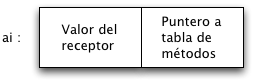
\includegraphics{oo/interface_value1.png} \end{center}
	
	En distintos momentos de la ejecución del programa posee distintos valores
	y tipo:
	
	\begin{verbatim} ai = &Punto { 3, 4 }  (== (*Punto) (0xff1234)):
	\end{verbatim}
	
	\begin{center} 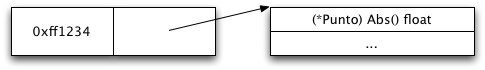
\includegraphics{oo/interface_value2.png} \end{center}
	
	\begin{verbatim} ai = MyFloat(-7.): \end{verbatim}
	
	\begin{center} 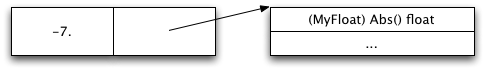
\includegraphics{oo/interface_value3.png} \end{center}
	
	\subsection{Hechos de los interfaces}
	
	Hay que tener en cuenta tres hecho sobre los interfaces en Go:
	
	\begin{enumerate} \item Los interfaces definen un conjunto de métodos. Son
	puros y completamente abstractos: No implementan nada, no tienen atributos.
	Go posee una clara separación entre interfaz e implementación.  \item Los
	valores de un interfaz son simplemente eso: valores. Contienen un valor
	concreto que implementa todos los métodos definidos en el interfaz.
	\textit{Dicho valor puede o puede no ser un puntero}.  \item Los tipos
	implementan interfaces simplemente teniendo sus métodos. No es necesario
	declarar explícitamente que lo hacen. Por ejemplo, como ya hemos visto,
	todos los tipos implementan \textit{EmptyInterface}.  \end{enumerate}
	
	\subsection{Ejemplo: io.Writer}
	
	El paquete \textit{io} concede una serie de métodos para el programador que
	pueden tratar la entrada y salida de datos. Para ver de forma más clara cómo
	son las interfaces, se ha elegido la interfaz \textit{io.Wirter} por ser
	bastante representativa y muy usada en Go.\\
	
	Si echamos un vistazo a la cabecera de la función \textit{Fprintf} del
	paquete \textit{fmt}, observamos que tiene la siguiente forma:
	
	\begin{verbatim} func Fprintf (w io.Writer, format string, a ...) (n int,
	error os.Error) \end{verbatim}
	
	Es decir, dicha función lo que recibe es una variable u objeto que sea de
	tipo io.Writer, no necesariamente un fichero donde escribir. El parámetro
	a de tipo ''...'' debería obviarse por ahora ya que se explicará más
	adelante. Como se puede observar, Fprintf devuelve una tupla con el número
	de caracteres escritos y el error en caso de que hubiera alguno.\\
	
	La interfaz io.Writer está definida de la siguiente manera:
	
	\begin{verbatim} type Writer interface { Write (p []byte) (n int, err
	os.Error) } \end{verbatim}
	
	Lo que quiere decir que todos los objetos que instancien dicha interfaz
	deberán tener un método Write que reciba un buffer de bytes y devuelva el
	número de caracteres escritos y un error en caso de que éste exista.\\
	
	Si echamos un vistazo al paquete \textit{bufio} que contiene métodos para
	realizar una entrada / salida con un buffer de datos, observamos que
	implementa un nuevo tipo de datos:

	\begin{verbatim} type Writer struct { ... } \end{verbatim}
	
	Implementando dicho tipo de datos (\textit{bufio.Writer}) el método
	\textit{Writer} canónico visto en el interfaz del mismo nombre.
	
	\begin{verbatim} func (b *Writer) Write (p []byte) (n int, err os.Error)
	\end{verbatim}
	
	Casi todos los paquetes de entrada / salida así como los que se encargan de
	la escritura en ficheros utilizan el interfaz Write. \\
	
	El paquete io tiene declarados 4 interfaces distintos, uno para cada uso
	distinto:
	
	\begin{itemize} \item Reader \item Writer \item ReadWriter \item
	ReadWriteCloser \end{itemize}
	
	\subsection{Comparación con C++}
	
	En C++ un tipo interfaz es como una clase abstracta pura, ya que se
	especifican los métodos pero no se implementa ninguno de ellos.\\
	
	En términos de Java, el tipo interfaz es mucho más parecido a una interfaz
	Java.\\
	
	En Go, hay una gran diferencia en un aspecto: Un tipo no necesita declarar
	las interfaces que implementa ni siquiera heredar de un tipo interfaz, sino
	que si tiene los métodos que definen el interfaz, entonces dicho tipo
	implementa el interfaz.
	
%	\subsection{Interfaces y atributos anónimos}	
	
%	\subsection{Ejemplo: Servicio HTTP}
	
	\subsection{Contenedores y la interfaz vacía}
	
	Los contenedores son estructuras de datos que permiten almacenar elementos
	de un determinado tipo o de cualquiera. Veamos cómo se realiza esto en una
	posible implementación de los vectores.  \clearpage \begin{verbatim} type
	Element interface {}
	   
	   //Vector es el propio contenedor type Vector struct { a []Element }
	   
	   // At() devuelve el i-ésimo elemento func (p *Vector) At(i int) Element
	   { return p.a[i] } \end{verbatim}
	
	Como se puede observar en el código anterior los vectores pueden contener
	elementos de cualquier tipo de datos ya que todos los tipos implementan la
	interfaz vacía (en este caso Element es una interfaz vacía). De hecho, cada
	elemento contenido en un vector podría ser de cualquier tipo.
	
	\subsection{Asertos de tipos}
	
	Una vez que se almacena un elemento en un \textit{Vector}, dicho elemento se
	almacena como un valor \textit{interfaz}. Es necesario por lo tanto
	``desempaquetarlo'' para tener el valor original, usando los asertos de
	tipos (o type assertions). Su sintaxis es:
	
	\begin{verbatim} valor_interfaz.(tipo_a_extraer) \end{verbatim}
	
	Veamos un ejemplo de cómo funcionarían los asertos:
	
	\begin{verbatim} var v vector.Vector
	   
	   v.Set (0, 1234.)  // Se guarda como un valor de interfaz i := v.At(0)
	   // Devuelve el valor como interface{}
	   
	   if i != 1234. {}            // Error en tiempo de compilación if
	   i.(float) != 1234. {}    // OK if i.(int) != 1234 {}       // Error en
	   tiempo de ejecución if i.(MyFloat) != 1234. {}  // Error: no es MyFloat
	   \end{verbatim}
	
	\subsection{Conversión de una interfaz a otra}
	
	Hasta ahora únicamente nos hemos limitado a mover valores normales dentro
	y fuera de valores interfaz, pero los valores de este tipo que contengan los
	métodos apropiados, también pueden ser convertidos a otros tipos de
	interfaces.\\
	
	De hecho, es lo mismo que desempaquetar el valor interfaz para extraer el
	valor concreto al que se hace referencia, para después volverlo a empaquetar
	para el nuevo tipo interfaz.\\
	
	La viabilidad de la conversión depende del valor referenciado, no del tipo
	original de la interfaz.\\
	
	Veamos un ejemplo de la conversión de intefaces, dadas las siguientes
	definiciones de variables y tipos:
	
	\begin{verbatim} var ai AbsInterface type SqrInterface interface { Sqr()
	float } var si SqrInterface pp := new(Point) // asumamos que *Point tiene
	Abs, Sqr var empty interface{} \end{verbatim}
	
	Todas estas operaciones serían correctas:
	
	\begin{verbatim} empty = pp  // Todo satisface empty ai
	= empty.(AbsInterface) // El valor referenciado // implementa Abs(). En
	cualquier otro // caso, produce un fallo en tiempo de ejecución.  si
	= ai.(SqrInterface)  // *Point tiene Sqr() // aunque AbsInterface no lo
	implemente empty = si // *Point implementa el conjunto vacío \end{verbatim}
	
	\subsection{Probando interfaces con asertos}
	
	En muchas ocasiones querremos saber con qué tipo de interfaz estamos
	tratando, es por ello que podemos gracias a los asertos preguntar qué tipo
	de interfaz tiene una determinada variable.\\
	
	Para ello se puede usar los asertos de tipo "coma ok":
	
	\begin{verbatim} elem := vector.At(0)
	   
	   if i, ok := elem.(int); ok { fmt.Printf ("int: \%d\n, i) } else if f, ok
	   := elem.(float); ok { fmt.Printf ("float: \%g\n", f) } else
	   { fmt.Print("tipo desconocido\n") } \end{verbatim} \clearpage También
	   podemos comprobar los interfaces con un switch de tipos:
	
	\begin{verbatim} switch v := elem.(type) {  // Literal "type" case int:
	fmt.Printf ("int: \%d\n", v) case float: fmt.Printf ("float: \%g\n", v)
	default: fmt.Print("tipo desconocido\n") \end{verbatim}
	
	Y yendo un paso más allá, podemos preguntar si un valor de tipo interfaz
	implementa un método. De esta forma, por ejemplo, es como \textit{Print}
	decide si el tipo puede imprimirse así mismo o si debe usar una
	representación genérica del mismo.
	
	\begin{verbatim} type Stringer interface { String() string }
	   
	   if sv, ok := v.(Stringer); ok { fmt.Printf("implementa String(): \%s\n",
	   sv.String()) } \end{verbatim}
	
	\subsection{El paquete reflect}
	
	En Go existe un paquete \textit{reflect} que utiliza la misma base de
	determinar los tipos de los parámetros en las llamadas a las funciones
	usando los asertos. Así es posible usar un nuevo argumento ''...'' que
	permite pasar argumentos indefinidos a una función. Veamos un ejemplo con
	\textit{Printf}:
	
	\begin{verbatim} func Printf (format string, args ...) (n int, err os.Error)
	\end{verbatim}
	
	El argumento ''...'' usado dentro de Printf (o en cualquier otro sitio)
	tiene el tipo \textit{interface\{\}}, y \textit{Printf} usa el paquete
	\textit{reflect} para desempaquetar y descubrir la lista de argumentos.\\
	
	Como resultado, tenemos que toda la familia de funciones \textit{Print}
	saben los tipos de todos sus argumentos. Como conocen si el argumento es
	unsigned o long, no hay necesidad de \textit{\%u} o \textit{\%ld},
	simplemente \textit{\%d}, simplificando mucho la lista de modificadores.
	


\chapter{Concurrencia y comunicación}

A medida que la informática avanza, se va haciendo más necesario el uso de
elementos de comunicación y concurrencia. La comunicación es algo necesario para
no formar parte de un sistema aislado, y así poder comunicar nuestro programa
con otros programas, que puede que estén o no en nuestra misma máquina.\\

La concurrencia, por otra parte, nos permite evitar situaciones indeseadas
y realizar programación paralela, haciendo que el aprovechamiento de los
recursos sea mucho más eficaz. Go es un lenguaje creado con dos fines: uno de
ellos es la simplicidad, y el otro es su eminente enfoque para sistemas
concurrentes.

\section{Goroutines}

	\subsection{Definición}
	
	Podríamos definir de manera formal una Goroutine como: \\

	\textit{''Una función de Go que permite ejecutar otra función de manera
	paralela al programa y en el mismo espacio de direcciones que realiza la
	llamada a la Goroutine.''}\\

	Todos los programas en Go constan de una o varias Goroutines.\\

	Aunque pueda llevar a confusión, una Goroutine no es lo mismo que un thread,
	un proceso, etc. Una Goroutine es una Goroutine.\\

	Evidentemente, y aunque pueda parecer un sistema perfecto, tiene sus
	problemas de concurrencia asociados que se irán viendo más adelante. Por
	ahora asumamos que funciona tal y como se ha dicho.  \clearpage
	\subsection{Cómo crear una Goroutine}
	
	Crear una Goroutine es quizá lo más sencillo que haya. Basta con invocar una
	función anteponiéndole la palabra reservada \textit{go}:
	
	\begin{verbatim} func IsReady (what strgin, minutes int64) { time.Sleep
	(minutes * 60 * 1e9) fmt.Println (what, "está listo") }
	   
		go IsReady ("té", 6) go IsReady ("café", 2) fmt.Println ("Estoy
		esperando...") \end{verbatim}
	
	El ejemplo anterior imprimiría:
	
	\begin{verbatim} Estoy esperando...   (de forma inmediata) café está listo
	(2 minutos después) té está listo        (6 minutos después) \end{verbatim}
	
	\subsection{Verdades de las Goroutines}
	
	Las Goroutines son baratas, es decir, son muy fáciles de programar y de
	invocar.\\
	
	Las Goroutines terminan su ejecución retornando de su función superior,
	o simplemente saliendo en algún punto intermedio del programa puesto a tal
	propósito. También pueden llamar a \textit{runtime.Goexit()}, aunque es
	raramente necesario.\\
	
	Las Goroutines pueden ejecutarse concurrentemente en diferentes procesadores
	con memoria compartida. Asimismo no hay por qué preocuparse del tamaño de la
	pila a la hora de invocarlas.
	
	\subsection{Pila de una Goroutine}
	
	En \textit{gccgo}, al menos por ahora, las goroutines se compilan como si
	fueran pthreads. Sus pilas son grandes. Se pretende cambiar esto en un
	futuro próximo pero no se ha realizado todavía ya que necesitan realizarse
	cambios en el propio \textit{gcc}.\\
	
	Usando el compilador \textit{6g}, las pilas son pequeñas (unos pocos kB)
	pero crecen a medida que sea necesario. De esta forma, las goroutines usan
	muy poca memoria pero si es necesario pueden de forma dinámica hacer crecer
	la pila para invocar a muchas más funciones.\\
	
	Esto se ha diseñado y programado así para que el programador no tenga que
	preocuparse sobre el límite de la pila y la tarea le resulte mucho más
	cómoda.
	
	\subsection{Scheduling}
	
	Las goroutines están multiplexadas entre múltiples threads del sistema.
	Cuando una goroutine ejecuta una llamada bloqueante al sistema, el resto de
	goroutines no se bloquean y continúan su ejecución.\\
	
	Se pretende realizar este mismo efecto para las goroutines dependientes de
	la CPU, pero por ahora si se quiere un paralelismo a nivel de usuario se
	necesita dar un valor a la variable de entorno \textit{\$GOMAXPROCS}, o se
	puede llamar en un programa a \textit{runtime.GOMAXPROCS(n)}.\\
	
	\textit{GOMAXPROCS} le dice al planificador en tiempo de ejecución cuántas
	goroutines que no sean bloqueantes por llamadas al sistema, pueden correr
	a la vez. Esto implica, que para hacer una prueba real de paralelismo,
	necesitaremos adecuar el valor de \textit{\$GOMAXPROCS} al número de
	goroutines que tenga nuestro programa.\\
	
	¿Cómo se puede dar un valor a dicha variable? Sencillo. En un terminal del
	sistema basta con poner las siguientes líneas:
	
	\begin{verbatim} $ GOMAXPROCS=4 $ export GOMAXPROCS \end{verbatim}

\section{Channels\label{channels}}

A menos que dos goroutines puedan comunicarse, éstas no pueden coordinarse
o sincronizarse de ninguna forma. Por ello Go tiene un tipo denominado
\textit{channel} que provee comunicación y sincronización. También posee de
estructuras de control especiales para los canales que hacen fácil la
programación concurrente.

	\subsection{El tipo channel}
	
	En su forma más simple el tipo se declara como:
	
	\begin{verbatim} chan tipo_elemento \end{verbatim}
	
	Dada una variable de ese estilo, puedes enviar y recibir elementos del tipo
	\textit{tipo\textunderscore elemento}.\\
	
	Los canales son un tipo de referencia, lo que implica que se pude asignar
	una variable \textit{chan} a otra y que ambas variables accedan al mismo
	canal. Esto también hace referencia a que hay que usar \textit{make} para
	alojar un canal:
	
	\begin{verbatim} var c = make (chan int) \end{verbatim} \clearpage
	\subsection{El operador $<-$}
	
	El operador $<-$ (más comúnmente conocido como ''flechita'') es un operador
	que nos permite pasar datos a los canales. La flecha apunta en la dirección
	en que se pretende que sea el flujo de datos.\\
	
	Como operador binario, $<-$ envía a un canal:
	
	\begin{verbatim} var c chan int c <- 1      // envía 1 al canal
	c \end{verbatim}
	
	Como un operador unario prefijo, $<-$ recibe datos de un canal:
	
	\begin{verbatim} v = <- c    // Recibe un valor de c y se lo asigna a v.  <-
	c        // Recibe un valor de c, descartándolo i := <- c   // Recibe un
	valor de c inicializando i \end{verbatim}
	
	\subsection{Semántica de canales}
	
	Por defecto la comunicación en Go se realiza de forma síncrona. Más tarde
	abordaremos la comunicacion asíncrona. Que la comunicación sea síncrona
	significa:
	
	\begin{enumerate} \item Una operación send en un canal bloquea la ejecución
	hasta que se ejecuta una operación receive en el mismo canal.  \item Una
	operación receive en un canal bloquea la ejecución hasta que una operación
	send es ejecutada en el mismo canal.  \end{enumerate}
	
	De esta forma, la comunicación es además una forma de sincronización:
	2 goroutines intercambiando datos a través de un canal, se sincronizan en el
	momento en que la comunicación es efectiva.
	
	\subsection{Ejemplo de comunicación}
	
	Veamos un ejemplo bastante tonto de comunicación pero que servirá como toma
	de contacto con la sintaxis de los canales:
	
	\begin{verbatim} func pump (ch chan int) { for i := 0; ; i++ { ch <- i } }
	   
		ch1 := make (chan int) go pump (ch1)       // pump se bloquea;
		ejecutamos: fmt.Println (<-ch1)     // Imprime 0
	   
	   
		func suck (ch chan int) { for { fmt.Println (<-ch) } }
	   
		go suck (ch1)    // Miles de números se imprimen
	   
		// Todavía se puede colar la función principal y pedir un valor
		fmt.Println(<-ch)    // Imprime un valor cualquiera (314159)
		\end{verbatim}
	
	\subsection{Funciones que devuelven canales}
	
	En el ejemplo anterior, \textit{pump} era una función generadora de valores
	para ser recogidos por otra función. El ejemplo anterior se puede
	simplificar bastante en el momento en el que se cree una función que pueda
	devolver el canal en sí para que se puedan recoger los datos.
	
	\begin{verbatim} func pump() chan int { ch := make (chan int) go func()
	{ for i := 0; ; i++ { ch <- i } }() return ch }
	   
		stream := pump() fmt.Println(<-stream)   // Imprime 0 \end{verbatim}
	
	\subsection{Rangos y canales}
	
	La claúsula \textit{range} en bucles \textit{for} acepta un canal como
	operando, en cuyo caso el bucle \textit{for} itera sobre los valores
	recibidos por el canal.\\
	
	Anteriormente reescribimos la función pump(), con lo que ahora reescribimos
	la función \textit{suck} para que lance la goroutine también:
	
	\begin{verbatim} func suck (ch chan int) { go func() { for v:= range ch
	{ fmt.Println(v) } }() }
	   
		suck (pump())   // Ahora esta llamada no se bloquea \end{verbatim}
	
	\subsection{Cerrando un canal}
	
	Cuando queremos cerrar un canal por alguna razón usamos una función del
	lenguaje que nos permite realizar dicha acción.
	
	\begin{verbatim} close (ch) \end{verbatim}
	
	De igual forma, existe otra función que nos permite comprobar si un canal
	está cerrado o no, usando la función \textit{closed()}:
	
	\begin{verbatim} if closed (ch) { fmt.Println ("hecho") } \end{verbatim}
	
	Una vez que un canal está cerrado y que todos los valores enviados han sido
	recibidos, todas las operaciones receive que se realicen a continuación
	recuperarán un valor ''cero'' del canal.\\
	
	En la práctica, raramente se necesitará \textit{close}.\\
	
	Hay ciertas sutilezas respecto al cierre de un canal. La llamada
	a \textit{closed()} sólo funciona correctamente cuando se invoca después de
	haber recibido un valor ''cero'' en el canal. El bucle correcto para
	recorrer los datos de un canal y comprobar si se ha cerrado es:
	
	\begin{verbatim} for { v := <-ch if closed (ch) { break } fmt.Println (v)
	} \end{verbatim}
	
	Pero de una forma mucho más idiomática y simple, podemos usar la cláusula
	\textit{range} que realiza esa misma acción por nosotros:
	
	\begin{verbatim} for v := range ch { fmt.Println (v) } \end{verbatim}
	
	\subsection{Iteradores}
	
	Ahora que tenemos todas las piezas necesarias podemos construir un iterador
	para un contenedor. Aquí está el código para un \textit{Vector}: \clearpage
	\begin{verbatim} // Iteramos sobre todos los elementos
	   
		func (p *Vector) iterate (c chan Element) { for i, v := range p.a {   //
		p.a es un slice c <- v } close (c)     // Señala que no hay más valores
		}
	   
		// Iterador del canal
	   
		func (p *Vector) Iter() chan Element { c := make (chan Element) go
		p.iterate (c) return c } \end{verbatim}
	
	Ahora que el \textit{Vector} tiene un iterador, podemos usarlo:
	
	\begin{verbatim} vec := new (vector.Vector) for i := 0 i < 100; i++
	{ vec.Push (i*i) }
	   
		i:= 0 for x := range vec.Iter() { fmt.Printf ("vec[\%d] is \%d\n", i,
		x.(int)) i++ } \end{verbatim}
	
	\subsection{Direccionalidad de un canal}
	
	En su forma más simple una variable de tipo canal es una variable sin
	memoria (no posee un buffer), síncrona y que puede ser utilizada para enviar
	y recibir.\\
	
	Una variable de tipo canal puede ser anotada para especificar que únicamente
	puede enviar o recibir:
	
	\begin{verbatim} var recv_only <-chan int var send_only chan <- int
	\end{verbatim}
	
	Todos los canales son creados de forma bidireccional, pero podemos
	asignarlos a variables de canales direccionales. Esto es útil por ejemplo en
	las funciones, para tener seguridad en los tipos de los parámetros pasados:
	
	\begin{verbatim}
	
	
		func sink (ch <- chan int) { for { <- ch } }
	   
		func source (ch chan<- int) { for { ch <- 1 } }
	   
		var c = make (chan) int)  //bidireccional go source (c) go sink (c)
		\end{verbatim}
	
	\subsection{Canales síncronos}
	
	Los canales síncronos no disponen de un buffer. Las operaciones send no
	terminan hasta que un receive es ejecutado. Veamos un ejemplo de un canal
	síncrono:
	
	\begin{verbatim} c := make (chan int) go func () { time.Sleep (60 * 1e9)
	x := <- c fmt.Println ("recibido", x) }()
	   
		fmt.Println ("enviando", 10) c <- 10 fmt.Println ("enviado", 10)
		\end{verbatim}
	
	Salida:
	
	\begin{verbatim} enviando 10  (ocurre inmediatamente) enviado 10   (60s
	después, estas dos lineas aparecen) recibido 10 \end{verbatim}

	\subsection{Canales asíncronos}
	
	Un canal asíncrono con buffer puede ser creado pasando a \textit{make} un
	argumento, que será el número de elementos que tendrá el buffer.
	
	\begin{verbatim} c := make (chan int, 50) go func () { time.Sleep (60 * 1e9)
	x := <-c fmt.Println ("recibido", x) }()
	   
	   
		fmt.Println ("enviando", 10) c <- 10 fmt.Println ("enviado", 10)
		\end{verbatim}
	
	\begin{verbatim} enviando 10  (ocurre inmediatamente) enviado 10   (ahora)
	recibido 10   (60s después) \end{verbatim}
	
	\textbf{Nota.-} El buffer no forma parte del tipo canal, sino que es parte
	de la variable de tipo canal que se crea.
	
	\subsection{Probando la comunicación}
	
	Si nos preguntamos si un receive puede en un momento determinado ejecutar
	sin quedarse bloqueado, existe un método que permite hacerlo de forma
	atómica, probando y ejecutando, utilizando para tal efecto el sistema ''coma
	ok''.
	
	\begin{verbatim} v, ok = <-c   // ok = true si v recibe un valor
	\end{verbatim}
	
	¿Y qué hay de realizar una operación send sin bloquear? Hace falta
	averiguarlo y ejecutar. Para ello usamos una expresión booleana:
	
	\begin{verbatim} ok := c <- v
	   
		o también:
	   
		if c <- v { fmt.Println ("valor enviado") } \end{verbatim}
	
	Normalmente, se quiere una mayor flexibilidad, que conseguiremos con la
	siguiente estructura que veremos en el uso de canales.

\section{Select}

	\subsection{Definición}
	
	\textit{Select} es una estructura de control en Go, análoga a un switch
	asociado a comunicación. En un \textit{select} cada case debe ser una
	comunicación: send o receive.
	
	\begin{verbatim} var c1, c2 chan int
	   
		select { case v := <- c1: fmt.Printf ("recibido \%d de c1\n", v) case
		v := <- c2: fmt.Printf ("recibido \%d de c2\n", v) } \end{verbatim}
	
	\textit{Select} ejecuta un case que pueda ejecutarse de forma aleatoria. Si
	ninguno de los case es posible de ejecutar, se bloquea hasta que uno lo sea.
	Una cláusula \textit{default} es siempre ejecutable.
	
	\subsection{Semántica de select}
	
	Hagamos un rápido resumen del select:
	
	\begin{itemize} \item Cada case debe ser una comunicación \item Todas las
	expresiones del canal son evaluadas \item Todas las expresiones para ser
	enviadas son evaluadas \item Si alguna comunicación puede producirse, se
	produce; En otro caso se ignora.  \begin{itemize} \item Si existe una
	cláusula \textit{default}, es ésta la que ejecuta \item Si no existe
	\textit{default}, el bloque select se bloquea hasta que una comunicación
	pueda realizarse; no hay reevaluación de los canales y/o posibles valores.
	\end{itemize} \item Si hay múltiples casos listos, uno es seleccionado
	aleatoriamente. El resto no ejecuta.  \end{itemize}
	
	\subsection{Ejemplo: Generador aleatorio de bits}
	
	Un ejemplo bastante ilustrativo es el siguiente:
	
	\begin{verbatim} c := make (chan int) go func() { for { fmt.Println (<-c)
	} }()
	   
		for { select { case c <- 0:   // No hay sentencias, no existe el
		fall-through case c <- 1: } } \end{verbatim}
	
	Esto imprime: 0 1 1 0 0 1 1 1 0 1 ...

\section{Multiplexación}

Los canales son valores de ''primer tipo'', es decir, pueden ser enviados
a través de otros canales. Esta propiedad hace que sea fácil de escribir un
servicio multiplexador dado que el cliente puede proporcionar, junto con la
petición, el canal al que debe responder.

\begin{verbatim} chanOfChans := make (chan chan int) \end{verbatim} \clearpage
O de forma más típica:

\begin{verbatim} type Reply struct { ... } type Request struct { arg1, arg2,
arg3 some_type replyc chan *Reply } \end{verbatim}

Vamos a ver un ejemplo cliente-servidor a lo largo de los siguientes puntos.

	\subsection{El servidor}
	
	\begin{verbatim} type request struct { a, b int replyc chan int }
	   
		type binOp func (a, b int) int
	   
		func run (op binOp, req *request) { req.replyc <- op(req.a, req.b) }
	   
		func server (op binOp, service chan *request) { for { req := <- service
		// Aquí se aceptan las peticiones go run(op, req) } } \end{verbatim}
	
	Para comenzar el servidor lo hacemos de la siguiente forma:
	
	\begin{verbatim} func startServer (op binOp) chan *request { req := make
	(chan *request) go server (op, req) return req }
	   
		var adderChan = startServer( func a, b int) int { return a + b })
		\end{verbatim} \clearpage \subsection{El cliente}
	
	\begin{verbatim} func (r *request) String() string { return fmt.Sprintf
	("\%d+\%d=\%d", r.a, r.b, <-r.replyc) } req1 := &request{ 7, 8, make (chan
	int) } req2 := &request{ 17, 18, make (chan int) }
	   
		adderChan <- req1 adderChan <- req2
	   
		fmt.Println (req2, req1) \end{verbatim}
	
	\subsection{La contrapartida}
	
	En el ejemplo anterior el servidor ejecuta en un bucle infinito, con lo que
	siempre está esperando peticiones. Para terminarlo de manera correcta, se le
	puede señalar con un canal. El siguiente servidor tiene la misma
	funcionalidad pero con un canal \textit{quit} para terminar el proceso.
	
	\begin{verbatim} func server (op binOp, service chan *request, quit chan
	bool) { for { select{ case req := <- service:  // Aquí se aceptan las
	peticiones go run(op, req) case <- quit: return } } } \end{verbatim}
	
	El resto del código es básicamente el mismo, sólo que con un canal más:
	
	\begin{verbatim} func startServer (op binOp) (service chan *request, quit
	chan bool) { req := make (chan *request) quit = make (chan bool) go server
	(op, service, quit) return service, quit }
	   
		var adderChan, quitChan = startServer( func a, b int) int { return
		a + b }) \end{verbatim}
	
	El cliente permanece inalterado ya que puede terminar el servidor cuando
	quiera con sólo ejecutar la sentencia:
	
	\begin{verbatim} quitChan <- true \end{verbatim}

\section{Problemas de concurrencia}

Como siempre que se programa de forma concurrente existen un montón de problemas
pero Go trata de hacerse cargo de ellos.\\

El envío y la recepción (operaciones send y receive) son atómicas. La sentencia
\textit{select} está programada y definida muy cuidadosamente para que no
contenga errores.\\

El problema viene principalmente dado porque las goroutines ejecutan en memoria
compartida, las redes de comunicacción pueden colapsarse, que no existen
debuggers multihilo...\\

El consejo por parte de los desarrolladores del lenguaje es no programar como si
estuviéramos en C o C++, o incluso Java.\\

Los canales dan sincronización y comunicación en una misma estructura, lo cual
los hace muy potentes, pero también hacen que sea fácil razonar si se están
usando de manera correcta o no.\\

La regla es:\\

\textit{``No comunicar programas con memoria compartida, sino compartir memoria
comunicándose''}\\

El modelo básico a la hora de programar utilizando la filosofía cliente-servidor
se resume en dos conceptos:

\begin{enumerate} \item Usar un canal para enviar datos a una goroutine dedicada
como servidor, ya que si una única goroutine en cada instante tiene un puntero
a los datos, no hay problemas de concurrencia.  \item Usar el modelo de
programación ``un hilo por cliente'' de forma generalizada, usado desde la
década de los 80 y que funciona bastante bien.  \end{enumerate}

\clearpage \thispagestyle{empty} \ \\ \newpage


\chapter{Modelo de Memoria de Go}

Este capítulo contiene información que afecta específicamente a la programación
concurrente en Go. Especialmente se centra en cómo afectan las operaciones a las
lecturas de datos de las variables en una goroutine de forma que se observe el
valor correcto producido por una escritura de la misma variable en otra
goroutine.

\section{Lo que primero ocurre}

En el ámbito de una única goroutine, las lecturas y escrituras deben comportarse
como si fueran ejecutadas en el orden especificado por el programa. Esto es, los
compiladores y procesadores pueden reordenar las lecturas y escrituras
ejecutadas en el ámbito de una única goroutine sólo cuando la reordenación no
cambia el comportamiento en esa goroutine definido por la especificación del
lenguaje. Debido a esta reordenación, el orden de ejecución observado por una
goroutine puede diferir del orden percibido por otra. Por ejemplo, si una
goroutine ejecuta \textit{a = 1; b=1;}, otra puede observar el valor actualizado
de \textit{b} antes que el de \textit{a}.\\

Para especificar los requisitos de lecturas y escrituras, definimos ''lo que
primero ocurre'', un orden parcial en la ejecución de operaciones de memoria en
un programa escrito en Go. Si el evento \textit{e$_1$} ocurre antes que otro
\textit{e$_2$}, entonces decimos que \textit{e$_2$} ocurre después que
\textit{e$_1$}. También, si \textit{e$_1$} no ocurre antes que \textit{e$_2$}
y no ocurre después que \textit{e$_2$}, entonces decimos que \textit{e$_1$}
y \textit{e$_2$} ocurren concurrentemente.\\

En una única goroutine, el orden de ''lo que primero ocurre'' es el orden
expresado en el programa.\\

La lectura \textit{r} de una variable \textit{v} puede observar una escritura
\textit{w} en \textit{v} si las siguientes dos afirmaciones ocurren:

\begin{enumerate} \item \textit{w} ocurre antes que \textit{r}.  \item No hay
otra escritura \textit{w} en \textit{v} que ocurra después de \textit{w} pero
antes que \textit{r}.  \end{enumerate}

Para garantizar que una lectura \textit{r} de una variable \textit{v} observa un
valor particular escrito por \textit{w} en \textit{v}, hay que asegurar que
\textit{w} es la única escritura que \textit{r} puede observar. Esto es,
\textit{r} está garantizado que lee la escritura \textit{w} si las siguientes
afirmaciones se cumplen:

\begin{enumerate} \item \textit{w} ocurre antes que \textit{r}.  \item Cualquier
otra escritura en la variable compartida \textit{v} ocurre o bien antes que
\textit{w} o bien después que \textit{r}.  \end{enumerate}

Este par de condiciones es más estricto que el primero; requiere que no haya
otras escrituras ocurriendo concurrentemente con \textit{w} o con \textit{r}.\\

En una única goroutine no existe concurrencia, así pues las dos definiciones son
equivalentes: una lectura \textit{r} observa el valor escrito por la escritura
más reciente \textit{w} en \textit{v}. Cuando varias goroutines acceden a una
variable compartida \textit{v}, deben utilizar eventos de sincronización para
establecer qué es lo que ocurre primero y así asegurar que las lecturas observan
los valores correctos de las variables compartidas.\\

La inicialización de una variable \textit{v} con el valor ''cero'' para el tipo
de \textit{v} se comporta como se ha definido en este modelo de memoria..\\

Las lecturas y escrituras de valores que ocupan más que el ancho de palabra de
la máquina, se comportan como varias operaciones del ancho de la palabra de
forma no especificada.

\section{Sincronización}

La sincronización entre las distintas goroutines es básica para que el programa
en cuestión pueda ejecutar correctamente y dar resultados satisfactorios.

	\subsection{Inicialización}
	
	La inicialización del programa se ejecuta en una única goroutine y las
	nuevas goroutines creadas durante la inicialización no comienzan su
	ejecución hasta que la inicialización termina.\\
	
	Si un paquete \textit{p} importa un paquete \textit{q}, la inicialización de
	las funciones de \textit{q} terminan antes de que empiece la inicialización
	de cualquiera de las de \textit{p}.\\
	
	La ejecución de la función \textit{main.main} comienza después de que todas
	las funciones \textit{init} hayan terminado.\\
	
	La ejecución de todas las goroutines creadas durante la ejecución de las
	funciones \textit{init} ocurre después de que todas las demás funciones
	\textit{init} hayan terminado.\\ \clearpage \subsection{Creación de
	Goroutines}
	
	La sentencia \textit{go} que comienza una nueva goroutine se ejecuta antes
	de que la ejecución de la propia goroutine comience. Veamos un ejemplo al
	respecto:
	
	\begin{verbatim} var a string
	    
		func f() { print (a) }
	    
		func hello() { a = ''Hello, World!" go f() } \end{verbatim}
	
	Una posible llamada a \textit{hello} imprimirá \textit{''Hello World!''} en
	algún momento en el futuro (quizá después de que \textit{hello} haya
	terminado).
	
	\subsection{Comunicación mediante canales}
	
	La comunicación mediante canales es el método principal de sincronización
	entre goroutines. Cada send en un canal particular se corresponde con un
	receive en ese mismo canal, que se ejecuta normalmente en otra goroutine.\\
	
	Un send en el canal se ejecuta antes de que la ejecución del receive
	correspondiente de dicho canal finalice.\\
	
	Este programa garantiza la impresión de \textit{''Hello, World!''}. La
	escritura de \textit{a} ocurre antes del send en \textit{c}, que ocurre
	antes de que el correspondiente receive en \textit{c} termine, cosa que
	ocurre siempre antes que \textit{print}.
	
	\begin{verbatim} var a string
	    
		func f() { a = ''Hello, World!" c <- 0 }
	    
		func main() { go f() <- c print (a) } \end{verbatim}
	
	\textit{Un receive de un canal sin buffer  ocurre siempre antes de que el
	send en ese canal termine}.\\
	
	El siguiente programa también garantiza que se imprime \textit{''Hello,
	World!}. La escritura en \textit{a} ocurre antes que el receive en
	\textit{c}, lo que ocurre antes de que se realice el correspondiente send
	\textit{c}, lo que ocurre antes de que se ejecute el \textit{print}.
	
	\begin{verbatim} var c = make (chan int) var a string
	    
		func f() { a = ''Hello, World!" <- c }
	    
		func main() { go f() c <- 0 print (a) } \end{verbatim}
	
	Si el canal tuviera buffer (por ejemplo, \textit{c = make (chan int, 1)})
	entonces el programa no podría garantizar la impresión de \textit{''Hello,
	World!''}. Puede imprimir la cadena vacía; No puede imprimir
	\textit{''Hello, sailor''}, aunque tampoco puede terminar de forma
	inesperada.

\section{Cerrojos - Locks}

El paquete \textit{sync} implementa dos tipos de cerrojos, \textit{sync.Mutex}
y \textit{sync.RWMutex}.\\

Para cualquier variable \textit{l} de tipo \textit{sync.Mutex}
o \textit{sync.RWMutex} y para n < m, la n-ésima llamada a \textit{l.Unlock()}
ocurre antes de que la m-ésima llamada a \textit{l.Lock()} termine.\\

El siguiente programa garantiza la impresión de \textit{''Hello, World!"}. La
primera llamada a \textit{l.Unlock()} (en \textit{f}) ocurre antes de que la
segunda llamada a \textit{l.Lock()} (en \textit{main}) termine, lo que ocurre
antes de que se ejecute \textit{print}.

\begin{verbatim} var l sync.Mutex var a string
    
	func f() { a = ''Hello, World!'' l.Unlock() }
    
	func main() { l.Lock() go f() l.Lock() print(a) } \end{verbatim}

Para cualquier llamada a \textit{l.RLock} en una variable \textit{l} de tipo
\textit{sync.RWMutex}, existe una n tal que la llamada a \textit{l.RLock}
termina después que la n-ésima llamada a \textit{l.Unlock} y su correspondiente
\textit{l.RUnlock} ocurre antes de la n+1-ésima llamada a \textit{l.Lock}.

\section{El paquete once}

El paquete \textit{once} provee de un mecanismo seguro para la inicialización en
presencia de varias goroutines. Múltiples threads pueden ejecutar
\textit{once.Do(f)} para una \textit{f} particular, pero sólo una de ellas
ejecutará la función \textit{f()} y el resto de llamadas se bloquearán hasta que
\textit{f()} haya terminado su ejecución.\\

\textit{Una única llamada a f() desde once.Do(f) termina antes de que cualquier
otra llamada a once.Do(f) termine}.\\

En el siguiente programa la llamada a \textit{twoprint} provoca que
\textit{''Hello, World!''} se imprima dos veces. La primera llamada
a \textit{twoprint} ejecuta \textit{setup} una vez.

\begin{verbatim} var a string
    
	func setup() { a = ''Hello, World!'' }
    
	func doprint() { once.Do(setup) print(a) }
    
	func twoprint() { go doprint() go doprint() } \end{verbatim}

\section{Sincronización incorrecta}

En este apartado se va a tratar los problemas más comunes que pueden darse en
una sincronización.\\

Nótese que una lectura \textit{r} puede observar el valor escrito por una
escritura \textit{w} que ocurre concurrentemente con \textit{r}. Aunque esto
ocurra, no implica que las lecturas que ocurran después de \textit{r} observen
escrituras que hayan ocurrido antes que \textit{w}.\\

En el siguiente programa puede ocurrir que \textit{g} imprima \textit{2} y luego
\textit{0}.  \clearpage \begin{verbatim} var a,b int
    
	func f() { a = 1 b = 2 }
    
	func g() { print(b) print(a) }
    
	func main() { go f() g() } \end{verbatim}

La realización de un doble intento de bloqueo para conseguir exclusión mutua, es
un intento de eliminar la sobrecarga de la sincronización. Por ejemplo, el
programa \textit{twoprint} puede ser escrito incorrectamente como se puede
observar a continuación, pero no garantiza que, en \textit{doprint}, observando
la escritura en la variable \textit{done} no implica observar la escritura en
\textit{a}. Esta versión puede (incorrectamente) imprimir una cadena vacía en
lugar de \textit{''Hello, World!''}.

\begin{verbatim} var a string var done bool
    
	func setup() { a = ''Hello, World!'' done = true }
    
	func doprint() { if !done { once.Do(setup) } print(a) }
    
	func twoprint() { go doprint() go doprint() } \end{verbatim} \clearpage Otro
	ejemplo de una mala sincronización es:

\begin{verbatim} var a string var done bool
    
	func setup() { a = ''Hello, World!'' done = true }
    
	func main() { go setup() for !done { } print(a) } \end{verbatim}
    
De la misma forma de antes no existe garantía que en \textit{main}, observando
la escritura en \textit{done} no implica observar la escritura en \textit{a},
así que este programa también puede imprimir la cadena vacía. Peor aún, no hay
garantías de que la escritura en \textit{done} sea observable desde
\textit{main}, dado que no hay eventos de sincronización entre los dos threads.
Asimismo el bucle en \textit{main} no garantiza su finalización.\\
    
Hay sutiles variantes en este tema, como este programa:

\begin{verbatim} type T struct { msg string }
    
	var g *T
    
	func setup() { t := new (T) t.msg = ''Hello, World!'' g = t }
    
	func main() { go setup() for g == nil { } print (g.msg) } \end{verbatim}

Incluso si el \textit{main} observa \textit{g != nil} y sale de su bucle, no hay
garantía de que observe el valor inicializado de \textit{g.msg}\\

Para terminar, veamos un pequeño ejemplo de una incorrecta sincronización
mediante canales. El siguiente programa, de la misma forma que los anteriores,
puede no imprimir \textit{''Hello, World!''}, imprimiendo una cadena vacía dado
que la goroutina no termina su ejecución antes de que lo haga el \textit{main}.

\begin{verbatim} var c chan int

	func hello() { fmt.Println(''Hello, World!'') c <- 0 }
    
	func main() { go hello() } \end{verbatim}

Dado que se realiza un send al canal pero no se realiza su receive
correspondiente en main, no se garantiza que hello termine de ejecutar antes de
que termine la ejecución de main, que aborta el programa.

% Anexo: Herramientas de Go
\chapter{Herramientas de Go}

\section{Compiladores}

Go viene con un conjunto de herramientas bastante completo. Entre las
herramientas más importantes, están los dos tipos de compiladores que podemos
usar para generar nuestros programas ejecutables: \emph{gccgo y 6g/8g}.\\

Vamos a ver características de uno y otro, y un ejemplo de cómo realizar una
compilación con el compilador nativo de Go, la versión 6g/8g. Una característica
común de ambos, es que generan un código únicamente entre un 10\% y un 20\% más
lento que código en C.

	\subsection{gccgo}
	
	El compilador \emph{gccgo} es un \textit{front-end} del famoso compilador
	de C, GCC. Posee las siguientes características:
	
	\begin{itemize} \item Es un compilador más tradicional.  \item Soporta
	32-bit y 64-bit bajo x86, además de ARM.  \item Genera muy buen código, pero
	no tan rápido como su hermano \emph{6g/8g}.  \item Se puede enlazar con
	GCC, y así realizar una compilación con C.  \item No soporta pilas
	segmentadas todavía y aloja cada goroutine - se verá más adelante - por hilo
	de ejecución.  \end{itemize}
	
	Su uso, es exactamente igual al uso que se le da a GCC, sólo que invocándolo
	con el comando gccgo.
	
	\subsection{6g/8g}
	
	El compilador \emph{6g/8g} es un compilador experimental nativo de Go.
	\emph{6g}, es el compilador asociado a la arquitectura amd64, y genera
	ficheros objeto con extensión ".6". \emph{8g}, es el compilador asociado
	a la arquitectura 386, y genera ficheros objeto con extensión ".8".
	\clearpage \begin{itemize} \item Es un compilador experimental.  \item
	Soporta 32-bit y 64-bit bajo x86, además de ARM.  \item Genera buen código
	de forma muy, muy rápida.  \item No se puede enlazar con GCC, pero tiene
	soporte FFI.  \item Posee un buen soporte de gouroutines, multiplexándolas
	en varios hilos de ejecución, e implementa las pilas segmentadas.
	\end{itemize}
	
	Para compilar un archivo cualquiera llamado \textbf{file.go}, usaremos el
	comando:
	
	\begin{verbatim} $ 6g file.go \end{verbatim}
	
	y para enlazar el archivo y así generar el fichero ejecutable
	correspondiente, usaremos:
	
	\begin{verbatim} $ 6l file.6 \end{verbatim}
	
	Finalmente, para ejecutar el programa usaremos el comando:
	
	\begin{verbatim} $ ./6.out \end{verbatim}
	
	\textbf{Nota.-} Hay que tener en cuenta, que si se usa la versión 32-bit del
	compilador, se cambiaría cada 6 por un 8.\\
	
	\textbf{Nota.-} Para conseguir compilar un fichero con su propio nombre (y
	así no usar el fichero ejecutable por defecto (6.out), podemos pasarle el
	parámetro \emph{-o fichero\textunderscore salida} (ejemplo: 6l -o fichero
	file.6).\\
	
	El \emph{linker} de Go (\textit{6l}), no necesita recibir ningún otro
	fichero del que dependa la compilación, como en otros lenguajes, ya que el
	compilador averigua qué ficheros son necesarios leyendo el comienzo del
	fichero compilado.\\
	
	A la hora de compilar un fichero \textbf{A.go} que dependa de otro
	\textbf{B.go} que depende a su vez de \textbf{C.go}:
	
	\begin{itemize} \renewcommand{\labelitemi}{-} \item Compila \textbf{C.go},
	\textbf{B.go} y finalmente \textbf{A.go}.  \item Para compilar
	\textbf{A.go}, el compilador lee \textbf{B.go}, no \textbf{C.go}
	\end{itemize}

\section{Otras herramientas}

La distribución de Go viene con una serie de herramientas bastante útiles,
aunque todavía le faltan otras importantes, como un depurador, que está en
desarrollo. Así pues, contamos con: Godoc, Gofmt y con gdb\footnote{Aquellos que
usen \emph{gccgo} pueden invocar \textit{gdb}, pero la tabla de símbolos será
como la de C y no tendrán conocimiento del \emph{run-time}}.

	\subsection{Godoc}
	
	\emph{Godoc} es un servidor de documentación, análogo a \textbf{javadoc},
	pero más fácil para el programador que éste último.\\
	
	Como comentamos al principio del manual, la documentación oficial de Go, que
	se puede ver en su página oficial\footnote{http://golang.org} se apoya
	precisamente en esta herramienta.\\
	
	Es una herramienta muy útil para generar la documentación de nuestros
	programas y poder compartirlo con la gente de forma rápida y sencilla,
	a través de la web.\\
	
	La documentación de las librerías estándar de Go, se basa en los comentarios
	del código fuente. Para ver la documentación de una librería, podemos verla
	online a través de la web \emph{http://golang.org/pkg} o bien a través de
	la linea de comandos, ejecutando:
	
	\begin{verbatim} godoc fmt godoc fmt Printf \end{verbatim}
	
	Y así cambiando \emph{fmt} por el nombre del paquete que queramos ver,
	y \emph{Printf} por la función en cuestión a ser visualizada.
	
	\subsection{Gofmt}
	
	\emph{Gofmt} es un formateador de código. Es una herramienta muy útil para
	ver correctamente el código. Todo el código que se puede observar en la
	página web oficial, está formateado con esta herramienta.
	
	%%%%%%%%%%%%%%%%%%%%%%
	% ¿Hablamos de la herramienta gotest?    %
	%%%%%%%%%%%%%%%%%%%%%%



\begin{thebibliography}{99}

\bibitem{Golang} The Go Authors. Go official web page. \url{http://golang.org}

\bibitem{PVanRoy} P. Van Roy. Programming Paradigms for Dummies: What Every
Programmer Should Know. \url{http://www.info.ucl.ac.be/~pvr/VanRoyChapter.pdf}

\bibitem{XCode} Apple. XCode. \url{http://developer.apple.com/xcode/}

\bibitem{MinGW} Joseph Poirier. Go mingw.
\url{https://bitbucket.org/jpoirier/go\_mingw/downloads/}, 2011.

\bibitem{MiekGieben} Miek Gieben. Learning Go v0.5.
\url{http://www.miek.nl/files/go/}. 2011

\bibitem{IBMGC} IBM. A Real-time Garbage Collector with Low Overhead and
Consistent Utilization. \url{http://www.research.ibm.com/people/d/dfb/papers.html}.

\bibitem{GoSpecOperators} The Go Authors. Go official specification: Operators.
\url{http://golang.org/doc/go\_spec.html#Operators}

\end{thebibliography}


\end{document}
